\documentclass{article} %basic LaTeX document type

%set capital Roman numeral section headings
%set capital Aramaic letters subsection headings
%set capital Arabic numbers subsubsection headings
\renewcommand\thesection{\Roman{section}.}
\renewcommand\thesubsection{\thesection\Alph{subsection}.}
\renewcommand\thesubsubsection{\thesubsection\arabic{subsubsection}.}

%set capital Roman numeral table numeration
\renewcommand*\thetable{\Roman{table}} 

%package needed for next lines
%makes section headings bold and upper case characters
%makes subsubsection headings in italics
\usepackage[explicit]{titlesec}
\titleformat{\section}{\bfseries}{\thesection}{1em}{\MakeUppercase{#1}}
\titleformat{\subsubsection}{\itshape}{\thesubsubsection}{1em}{#1}


%\linespread{2}       %option 1 for making text double-spaced
\usepackage{setspace} %option 2 for making text double-spaced
\doublespacing

%makes first paragraph of section indented (non-first are by default)
%set size of indentation (15pt is default)
\usepackage{indentfirst}
\setlength{\parindent}{25pt}

%set size of all margins
\usepackage[margin=1.3in]{geometry}
%can set margin sizes which are not the same in this way
%\usepackage[left=1in, top=1in, right=1in, bottom=1in]{geometry}

%package which returns number of last page (same as number of pages)
%package which counts the number of tables and/or figures
\usepackage{lastpage}
\usepackage[figure,table]{totalcount}

%enable `align' equation types
%enable `multirow' capability in tables
%enable figures
\usepackage{amsmath}
\usepackage{multirow}
\usepackage{graphicx}

%enables double spaced footnotes
\usepackage[]{footmisc}

%enables subfigures
%enables subfigure captions
%sets table caption formatting options to meet NSE requirements
%sets figure caption options to meet NSE requirements
\usepackage{caption}
\usepackage[labelformat=simple]{subcaption}
\captionsetup[table]{labelsep=newline,name=TABLE}
\captionsetup[figure]{name=Fig.,labelsep=period}

%sets labeling of footnotes
%double spacing of footnotes
\renewcommand{\thefootnote}{\alph{footnote}}
\renewcommand{\footnotelayout}{\doublespacing}

%enables proper labeling of subfigures
\renewcommand*\thesubfigure{(\alph{subfigure})}

%--------------
\usepackage{paralist}	
\usepackage{amssymb}
\usepackage{epsfig}
\usepackage[mathcal]{euscript}
\usepackage{setspace}
\usepackage{color}
\usepackage{array}
%\usepackage{subfigure}
\renewcommand{\ttdefault}{cmtt}
% The float package HAS to load before hyperref
\usepackage{float} % for psuedocode formatting
\usepackage{xspace}
\usepackage{mathrsfs}
\usepackage[pdftex,hidelinks]{hyperref}
\usepackage[super]{nth}
\usepackage[export]{adjustbox}
\usepackage{placeins} % for float barriers
\usepackage{stmaryrd} % for short right arrow

%-------------
\newcommand{\bo}{\mathbf\Omega}
\newcommand{\vecr}{\textbf{r}}
\newcommand{\sn}{S$_\mathrm{N}$}
\newcommand{\pn}{P$_\mathrm{N}$}
\newcommand{\ve}[1]{\ensuremath{\mathbf{#1}}}
\newcommand{\xbar}{\ensuremath{\bar{x}}}
\newcommand{\qhat}{\ensuremath{\hat{q}}}
\newcommand{\E}[1]{$\times10^{#1}$}
\newcommand{\fwc}{\mbox{FW-CADIS}}
\newcommand{\Ye}[2]{\ensuremath{Y^e_{#1}(\bo_#2)}}
\newcommand{\Yo}[2]{\ensuremath{Y^o_{#1}(\bo_#2)}}
\newcommand{\sa}{\shortrightarrow}
\newcommand{\co}{\mbox{CADIS-$\Omega$}}
\newcommand{\mr}[1]{\multirow{2}{*}{#1}}

\begin{document}

%Define fields for \maketitle  (fields are \author, \date, \thanks, and \title)

\title{Assessment of the Lagrange Discrete Ordinates Equations for Monte Carlo Variance
Reduction Parameter Generation} %title of paper

\author{
\vspace{20mm}
%list of authors, with corresponding author marked by asterisk
\\Kelly L.\ Rowland,$^{\text{a}}$  Cory D.\ Ahrens,$^\text{b}$ Steven Hamilton,$^\text{c}$ 
\\and R.N.\ Slaybaugh$^{\text{a},\ast}$\\[4pt] 
%affiliations of authors
\textit{$^a$University of California, Berkeley, Nuclear Engineering Department}\\[-10pt]
\textit{4173 Etcheverry Hall, Berkeley, CA 94720, USA} \\[-5pt]
\textit{$^b$X Theoretical Design Division, Primary Physics Group}\\[-10pt]
\textit{Los Alamos National Laboratory, Los Alamos, NM 87545, USA}\\[-5pt]
\textit{$^c$Oak Ridge National Laboratory, Radiation Transport and Criticality Group} \\ [-10pt]
\textit{P.O. Box 2008, Oak Ridge, TN 37831-6170, USA} \\ [-2pt]
{$^\ast$slaybaugh@berkeley.edu}}       %address and email address for correspondence

%instead of returning the date, this repurposes the \maketitle command to print the number of pages, tables, and figures
\date{
\vspace{40mm}
Number of pages: \pageref{LastPage} \\  
Number of tables: \totaltables \\
Number of figures: \totalfigures \\}

\maketitle

\pagebreak

\begin{abstract} {

Hybrid radiation transport methods that use deterministic solutions to speed
up stochastic calculations are rarely effective for shielding problems with
highly anisotropic particle movement and particle streaming pathways. In this
work, we investigate using a different deterministic formulation, the Lagrange
Discrete Ordinates (LDO), for variance reduction parameter generation in
hybrid methods.  The LDO equations retain the formal structure of the
traditional discrete ordinates approximation of the Boltzmann transport
equation while handling the angular variable and particle scattering in a
unique fashion. The LDO equations' solutions have an interpolatory structure
such that the angular flux can be naturally evaluated at directions other than
the discrete ordinates used in arriving at the solutions, and those discrete
ordinates at which the problem is solved may be chosen in a strategic way. Of
particular interest is that the LDO equations have been shown to mitigate ray
effects at increased angular resolutions. Here, we assess the LDO equations'
scalar flux solutions as input in the CADIS and \fwc\ methods for Monte Carlo
variance reduction parameter generation. Monte Carlo calculations and Figures
of Merit using biasing parameters from the LDO equations are compared against
those using biasing parameters from standard quadrature set types for a small
variety of test case scenarios in both neutron and photon transport. The LDO
equations' variance reduction parameters see their best performance in the
\fwc\ method, especially for photon transport.

Keywords: hybrid methods; transport; Lagrange discrete ordinates
}
\end{abstract}

\pagebreak

%%---------------------------------------------------------------------------%%
\section{Introduction}
\label{sec:intro}

Radiation shielding is an important and interesting problem from various
perspectives. Simulation of shielding scenarios is critical for health physics
and nuclear security applications, but arriving at a solution for a given
response of interest (e.g., neutron flux at a given location) can be
computationally difficult in the context of the magnitude of particle
attenuation often seen in shielding problems.

The steady-state Boltzmann transport equation, shown below in Equation
\eqref{eq:bte}, is typically solved using either deterministic methods or
stochastic (Monte Carlo) methods.
%
\begin{multline}
\bo \cdot \nabla \psi(\vecr,E,\bo) + \Sigma_t(\vecr,E) \psi(\vecr,E,\bo) = \\
\int_0^\infty\int_{4\pi} \Sigma_s(\vecr,E'\rightarrow E,\bo'\cdot\bo)
\psi(\vecr,E',\bo')d\bo'dE' + Q(\vecr,E,\bo)
\label{eq:bte}
\end{multline}
%
So-called ``hybrid'' methods aim to combine the favorable aspects of
deterministic and Monte Carlo methods to achieve more accurate results more
quickly. The CADIS (consistent adjoint driven importance sampling) and \fwc\
(forward-weighted CADIS) methods are the current state of the art in Monte
Carlo variance reduction parameter generation for shielding. However, these
methods do not entirely mitigate the negative aspects of the combined
simulation types.

One particular area of interest where even hybrid methods struggle to yield
accurate results quickly is in shielding problems with highly anisotropic
particle movement and particle streaming pathways. This is because the
standard implementation of the CADIS and \fwc\ methods is based on scalar
particle flux rather than angular particle flux. So, solutions from
deterministic calculations exclude information about how particles move toward
a response of interest. For problems with strong anisotropies in the particle
flux, the importance map and biased source  developed using the standard
space/energy treatment may not represent the real importance well enough to
sufficiently improve efficiency in the Monte Carlo calculation.

This work aims to gauge the performance of Monte Carlo biasing parameters
based on scalar flux solutions from solving the Lagrange Discrete Ordinates
(LDO) equations.  We employ the LDO equations' solutions in the standard CADIS
and \fwc\ methods to assess how well the LDO representation's unique treatment
of scattering and asymmetry in angle incorporate angular information into the
resultant scalar flux solutions and corresponding Monte Carlo biasing
parameters. Deterministic calculations were performed with the Denovo
radiation transport code developed by Oak Ridge National Laboratory
\cite{denovo} in the Exnihilo framework, with Monte Carlo biasing parameters
generated via the ADVANTG software \cite{advantg} and Monte Carlo calculations
run with MCNP5 \cite{mcnp}.

The remainder of the paper is structured as follows: background information is
given regarding the CADIS and \fwc\ methods as well as about the LDO
equations. Test case scenarios are then described with relevant calculation
parameters listed; numerical results and discussion follow. We conclude with a
summary of the results and a discussion of suggested pathways for future work.

%%---------------------------------------------------------------------------%%
\section{Background}
\label{sec:background}

Here we begin by describing the CADIS (consistent adjoint driven importance
sampling) and \fwc\ (forward-weighted CADIS) methods, which are the current
state of the art of Monte Carlo variance reduction parameter generation. A
brief introduction to the LDO equations is then given to demonstrate
the difference between the LDO representation and the classical discrete
ordinates (\sn) equations.

%%---------------------------------------------------------------------------%%
\subsection{CADIS and \fwc}

%%---------------------------------------------------------------------------%%
\subsubsection{CADIS}

The CADIS method was introduced by Wagner and Haghighat to automate Monte
Carlo variance reduction parameter generation \cite{cadis}. CADIS is based on
the source biasing and weight window techniques, does not depend heavily on
user experience, and was first implemented as described in Reference
\cite{cadis} in the MCNP code. Most importantly, the result of using the CADIS
method is source biasing parameters and weight window target values such that
particles are born with the target weights. The CADIS method is very effective
for automated optimization of localized response values.

Using this method, source particles' energy and position are sampled from the
biased source distribution
%
\begin{equation}
\qhat(\vecr,E) = 
\frac{\phi^{\dagger}(\vecr,E)q(\vecr,E)}
{\int_V\int_E\phi^{\dagger}(\vecr,E)q(\vecr,E) dE\ d\vecr} 
= \frac{\phi^{\dagger}(\vecr,E)q(\vecr,E)}{R},
\label{eq:cadis_sb}
\end{equation}
%
where $\phi^{\dagger}$ denotes the adjoint scalar neutron flux, $q$
is the particle source density, and $R$ is some response of interest.

A key result of the CADIS method is that the statistical weights of
the source particles are the weight windows centers. In other
words, the source-biasing parameters and the weight window target values are
consistent. This circumvents the potential of particles being immediately split
or rouletted upon birth and avoids the resultant degradation in computational
efficiency. We refer the reader to Reference \cite{cadis} for a complete
discussion of results and analysis of the initial implementation of the CADIS
method. The CADIS method is very effective for automated optimization of
localized detectors but falls short of efficiently optimizing distributed
responses. \fwc, discussed in the next section, was developed to address this
issue.

%%---------------------------------------------------------------------------%%
\subsubsection{\fwc}

\fwc\ is a variation on the CADIS method to increase the efficiency of Monte
Carlo calculations of distributions and responses at multiple localized
detectors \cite{fwcadis}. For this global variance reduction method, a
response with uniformly-low statistical uncertainty across all phase-space is
desired. One way to target this for a given Monte Carlo simulation is to
uniformly distribute the particles throughout the system. Though this is not a
physical response, it is a proxy for the goal of obtaining uniform
uncertainty. It also indicates the possibility of developing an adjoint
importance function that represents the importance of particles to achieving
the goal of uniform particle distribution.

With this new problem formulation, the adjoint source is defined as
%
\begin{equation}
q^{\dagger}(\vecr,E,\bo) = \frac{1}{\psi(\vecr,E,\bo)},
\end{equation}
%
where $\psi$ denotes the angular neutron flux. From this,
we can calculate an adjoint importance function that represents the
importance of particles to achieving the desired objective of uniformly
distributed Monte Carlo particles. This should, in turn, correspond to
approximately uniform statistical uncertainties. The method physically 
corresponds to weighting the adjoint source with the inverse of the forward
flux; the adjoint source will be high where the forward flux is low and the
adjoint source will be low where the forward flux is high. With this method,
after the adjoint has been determined, the standard CADIS procedures are used
to calculate consistent source biasing parameters and weight windows.

%%---------------------------------------------------------------------------%%
\subsection{Classical Discrete Ordinates (\sn) Equations}

When solving the steady-state Boltzmann transport equation using deterministic
methods, as is done in the initial phase(s) of a hybrid methods calculation, the
discrete ordinates, or \sn, approximation is the most commonly-used
discretization for angle. This approximation gives one equation for each angle,
index $n$:
%
\begin{multline}
\bo_n \cdot \nabla \psi_n^g(\vecr) + \Sigma_t^g(\vecr)\psi_n^g(\vecr) = \\
\sum_{g'=0}^{G-1}\sum_{\ell=0}^{P}\Sigma_{s,\ell}^{g'\sa g}(\vecr)
\bigg[\Ye{\ell 0}{n}\phi_{\ell 0}^{g'}(\vecr) + \sum_{m=1}^{\ell}
\bigg(\Ye{\ell m}{n}\phi_{\ell m}^{g'}(\vecr) \\
 + \Yo{\ell m}{n}\vartheta_{\ell m}^{g'}(\vecr)\bigg)\bigg]
+ Q_n^g(\vecr),
\label{eq:sn}
\end{multline}
%
where a standard multigroup energy approximation is used ($G$ is the
number of discrete energy groups corresponding to the discretization index
$g$). The scattering term is expanded in terms of spherical harmonics
$\Ye{\ell m}{n}$ and $\Yo{\ell m}{n}$; $\phi$ and $\vartheta$ are the
``flux moments'' that are eventually used to  solve for the scalar flux
solution. The upper limit of summation for the scattering term spherical
harmonic expansion, denoted as $P$ in Eq. \eqref{eq:sn}, is known as the
``\pn\ order''.

Angular integration is approximated with the quadrature rule 
%
\begin{equation}
\int_{4\pi} f\left(\bo\right) d\bo \approx \sum_{n=1}^{N}w_n f\left(\bo_n\right)\:,
\label{eq:quadrule}
\end{equation}
%
where $w_n$ are the integration weights and $N$ is the number of ordinates.
We refer the reader to Reference
\cite{denovo} and the references therein for a complete discussion of the
derivation of the \sn\ equations as well as solution methods for the equations.

%%---------------------------------------------------------------------------%%
\subsection{Lagrange Discrete Ordinates (LDO) Equations}

The Lagrange Discrete Ordinates (LDO) equations are formally the same as the
classical \sn\ equations and are written for each discrete angle in the angle
set as
%
\begin{multline}
\bo_n\cdot\nabla\psi_{n}(\vecr,E) + 
\Sigma_{t}(\vecr,E)\psi_{n}(\vecr,E) = \\
\int_0^\infty\sum_{m=1}^{N}\sum_{n'=1}^{N}\langle L_{n'},L_{m}\rangle
\Sigma_{s,L}(\vecr,E'\rightarrow E)(\bo_{m}\cdot\bo_n)\psi_{n'}(E')dE'
+ Q_{n}(E),
\end{multline}
%
where $N$ is the number of discrete angles used in the formulation
and is a property of the maximum degree of integration of the quadrature set
on which the equations are based, $L_n$ is the $n^{th}$ Lagrange function, and
$\Sigma_{s,L}$ is the scattering cross section restricted to maximum degree
$L$. A full derivation can be found in Reference \cite{ahrens}.

The notable differences between the LDO equations and the classical \sn\
equations can be summarized as:

\begin{enumerate}
\item{The LDO equations' solutions have an interpolatory structure in angle,
      which allows the angular flux to naturally be evaluated at directions
      other than those in the discrete ordinates used to construct and solve
      the equations.}
\item{The LDO formulation does not require calculation of spherical harmonic
      moments.}
\item{The positive-weight quadrature sets on which the LDO equations are based
      can integrate spherical harmonics ranging from degree 0 to degree 165.}
\end{enumerate}

For a given fixed maximum degree of integration $L$, the corresponding number
of ordinates in the LDO formulation is $(L+1)^2$. The LDO equations are
developed with and must be evaluated at a fundamental system of points for the
subspace of spherical harmonics. Ahrens provides references for examples of
construction methods of these point systems \cite{ahrens}. As in the 
fundamental studies of the LDO equations conducted by Ahrens, we
have chosen to use the extremal point sets developed and distributed by
Womersley \cite{wom}.

%%---------------------------------------------------------------------------%%
\subsection{Previous Work}

Substantial effort has been placed into the development and automated
execution of hybrid methods. This section will discuss previous work in this
field with a  particular emphasis on hybrid methods  that incorporate neutron
direction of travel. As CADIS and \fwc\ are the current state of the art in
Monte Carlo variance reduction parameter generation, we will see that the
angle-informed hybrid methods are generally variants of CADIS and \fwc.

Noting the marked performance of the CADIS and \fwc\ methods, their limited
implementation in only space and energy, and the importance of particle
direction, Peplow introduced directional CADIS in 2012 \cite{peplow}. Two
versions of directional CADIS were explored: one method that biases the source
in space and energy while preserving the original angular distribution of the
particles, and one method that biases the source in space, energy, and angle.
Both new methods were tested against standard CADIS for seven example
problems, with the Monte Carlo calculation Figure of Merit (FOM), defined
below in Equation \eqref{eq:fom}, compared among the methods for each problem.
For most of these problems, directional CADIS outperformed standard CADIS,
increasing the Monte Carlo FOM by a factor of around 2. Notable cases in which
directional CADIS performed more poorly than standard CADIS are a neutron
porosity tool problem and a gamma-ray litho-density tool problem with the
detector far away from the source. It should also be noted that, for a
spherical boat test problem with a source far away from the boat, both
standard CADIS and directional CADIS performed more poorly than an analog
Monte Carlo calculation. For full details on the test results, we refer the
reader to Reference \cite{peplow}. In the conclusions of the report, Peplow
notes that ``it is difficult to know \textit{a priori} which problems would
benefit  from the space/energy/angular treatments presented in this work more
than from just using the standard space/energy CADIS.''

One of the most recent developments in the area of angle-informed hybrid
methods is \co, introduced by Munk et al.\ in 2016 \cite{cadisom}. This method
calculates an alternative form of the adjoint scalar flux quantity that is then
used in the CADIS and \fwc\ methods for generation of variance reduction
parameters for local and global response functions, respectively. The \co\
method was implemented in the ADVANTG framework, with numerical experiments
performed testing variance reduction for problems run in MCNP5. Several
characterization problems with spatially-induced anisotropies were tested to
evaluate the new method when used with CADIS and \fwc. Munk identified three
categories of processes that affect particle flux  anisotropy: strongly
directional particle sources, strong differences between material properties,
and algorithmic limitations that result in ray effects. Having grouped these
processes, Munk tested a set of characterization problems, each of which have
different combinations of the above anisotropy-inducing mechanisms. Munk also
developed a set of metrics by which the anisotropy of the flux may be
quantified over the various problems. Similar to the conclusions drawn by
Peplow, Munk found that it was difficult to predict for which problems \co\
should outperform CADIS. When considering a parametric study of deterministic
variables likely to affect angular flux (varying quadrature set order and \pn\
order) in a characteristic problem composed of a steel beam embedded in
concrete, \co\ achieved higher FOM values than standard CADIS for all
quadrature and \pn\ orders at high energies. Similarly, for a simple labyrinth
geometry of an air maze through a concrete block, \co\ achieved lower relative
errors than did standard CADIS in the epithermal and fast neutron energy
groups.

There have been several other efforts to improve variance reduction techniques
for problems with strong particle streaming anisotropies such as AVATAR
(Automatic Variance And Time of Analysis Reduction) \cite{avatar}, Cooper and
Larsen's Weight Windows \cite{clww}, and LIFT, the local importance function
transform \cite{lift1, lift2}. See Reference \cite{kr} for more detail. The
conclusions of these research efforts have been that methods either work
predictably but are complex to use, putting a high burden on user expertise,
or are simple to use but do not consistently perform well.

%%---------------------------------------------------------------------------%%
\section{Test Cases and Calculation Parameters}

In this section we introduce and describe the test case scenarios examined as
well as the various parameters chosen for the calculations in this work.
First, we present descriptions of the geometry and materials used in the test
cases as well as why each problem was chosen. Then, we discuss the parameters
chosen for the various deterministic and Monte Carlo calculations performed in
this work.

%%---------------------------------------------------------------------------%%
\subsection{Steel Plate Embedded in Water}
\label{sec:steel_params}

The first test case we describe is an idealized geometry of a steel plate 
embedded in water; it is modeled after the scenario presented in Reference 
\cite{wilsonslaybaugh}. This idealized geometry is of interest because it has
been shown to be computationally challenging: resonances in the iron cause
self-shielding in energy, and spatial self-shielding comes from the presence
of a thin plate of resonance material embedded in a moderating material. In 
turn, Monte Carlo variance reduction parameters generated from deterministic
solutions exhibit slow Monte Carlo error reduction.
A diagram of the problem geometry is shown in Figure \ref{steelxz} and a list
of material properties used in the problem is given in Table \ref{steel-mat}.
In Figure \ref{steelxz}, the orange region contains the source material, the 
black region is composed of steel, the blue regions indicate water, and the 
white region is composed of air.

\begin{figure}[!htb]
\centering
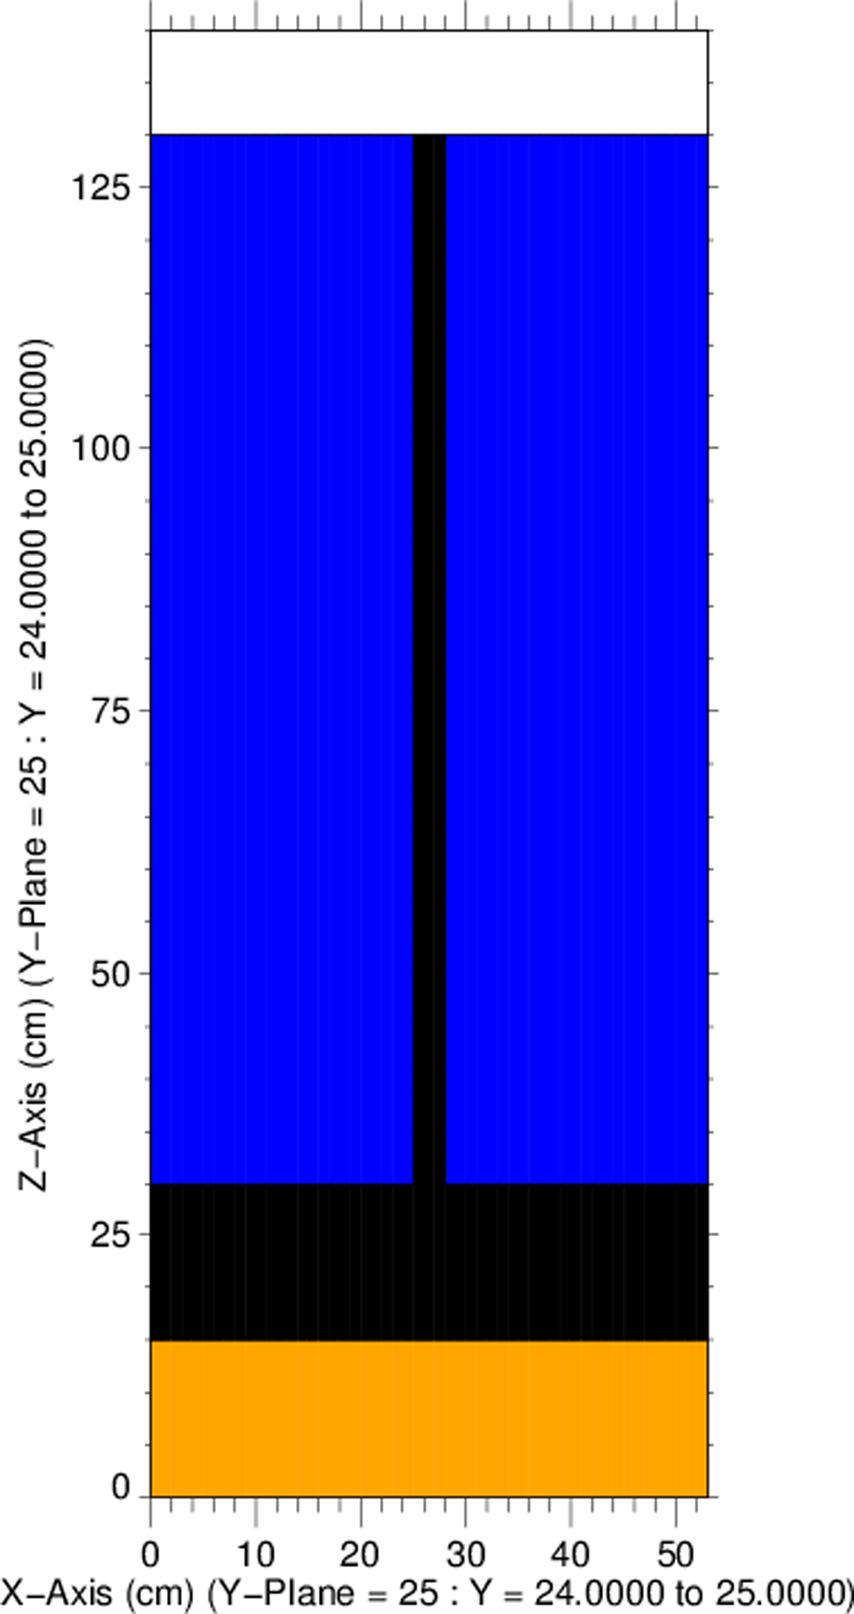
\includegraphics[width=0.4\textwidth]{img/steel-xz.png}
\caption{Steel plate in water geometry ($x-z$ slice through $y = 25$ cm) 
         \cite{wilsonslaybaugh}.}
\label{steelxz}
\end{figure}

The problem measurements are $53\times50\times140$ cm. The scenario is uniform 
in the $y$-direction and materials vary mainly in the $z$-direction. The source
region extends from 0 to 15 cm, the steel shield extends between 15 and 30 cm, 
the water and steel plate extend from 30 to 130 cm, and the air extends from 
130 to 140 cm. The steel plate is 3 cm wide and is centered at $x = 26.5$ cm. 
Vacuum boundary conditions were used at the problem boundaries.

A non-uniform Cartesian mesh was used for the spatial discretization in the 
deterministic calculations. In the $x$-direction, voxel width is 5 cm between
$x = 0$ cm and $x = 25$ cm, 0.5 cm between $x = 25$ cm and $x = 28$ cm, and 5 
cm between $x = 28$ cm and $x = 53$ cm. A uniform spacing of voxel width 1 cm 
was used in the $y$-direction. In the $z$-direction, the spatial cell width is
3 cm between $z = 0$ cm and $z = 30$ cm and 2 cm between $z = 30$ cm and 
$z = 140$ cm.

\begin{table}[!htb]
\centering
\caption{Materials and compositions in the steel plate in water scenario.}
\label{steel-mat}
\begin{tabular}{l|cc}
\textbf{Material} & \multicolumn{2}{c}{\textbf{Isotopes (Atomic \%)}} \\ \hline
\multirow{5}{*}{Source}   & U-235   & (0.000247) \\
                          & U-238   & (0.009287) \\
                          & Zr-nat. & (0.004009) \\
                          & H-1     & (0.037394) \\
                          & O-16    & (0.034927) \\ \hline
\multirow{4}{*}{Air}      & N-14    & (0.784431) \\
                          & O-16    & (0.210748) \\
                          & Ar-nat. & (0.004671) \\
                          & C-nat.  & (0.000150) \\ \hline
\multirow{2}{*}{Carbon Steel} & C-nat.  & (0.022831) \\
                              & Fe-nat. & (0.977169) \\ \hline
\multirow{2}{*}{Water}        & H-1     & (2)        \\
                              & O-16    & (1)        \\
\end{tabular}
\end{table}

The composition of the neutron source block is a homogenization of water,
zirconium, and uranium and was calculated based on the geometry and
composition of the Rowlands UO$_2$ pin cell benchmark specification
\cite{pincell}. The source is a U-235 fission  spectrum that is uniformly
distributed throughout the homogenized material. The compositions of air,
carbon steel, and water were taken from the Compendium of  Material
Composition Data for Radiation Transport Modeling \cite{pnnl}. For this
scenario, we are interested in the flux solutions at the end of the steel plate.

%%---------------------------------------------------------------------------%%
\subsection{Dog-Legged Void Neutron (DLVN)}

The next problem modeled is the dog-legged void neutron (DLVN) experimental 
benchmark, which was designed to measure neutron streaming in iron with air
voids. The model used in the following calculations was constructed from
References \cite{sw-dlvn,j-dlvn,dlvn1991}. The two materials used in the
problem are elemental iron and polyethylene. The polyethylene composition used
was C$_2$H$_4$. This is listed as ``polyethylene, non-borated'' and is material
248 in Reference \cite{pnnl}. 

\begin{figure}[!htb]
\centering
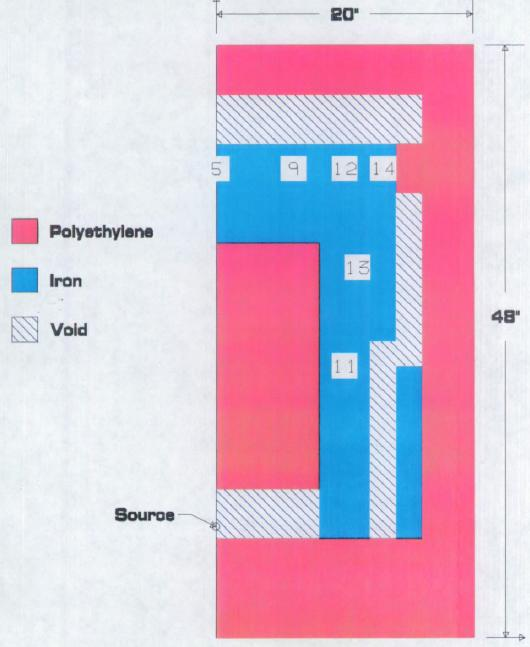
\includegraphics[width=0.5\textwidth]{img/dlvn.png}
\caption{Centerline cutaway of DLVN setup \cite{sw-dlvn}.}
\label{dlvn}
\end{figure}

The problem measurements are $40\times54\times48$ inches. A uniform spatial
mesh was imposed over the entire problem, with voxels measuring 1 inch per
side. The neutron source in this problem is a Cf-252 point source located at
the center of the $x-$ and $y-$directions and at $z = 9$ inches. This point
source was approximated as a small volumetric source in the tests in this
work. We are interested in the forward flux solutions at the various detector
locations shown in Figure \ref{dlvn}; this test case scenario is of interest 
because the streaming pathways in the configuration make the problem computationally
challenging. Additionally, the availability of experimental flux solution data
provides actual values against which to compare the calculated solutions.

The experimental configuration is symmetric about the $y-z$ plane at $x = 0$
and so is usually simulated with a reflecting boundary at $x = 0$ and vacuum
boundaries on all other sides of the configuration. For the tests in this work,
the use of reflecting boundary conditions was not available, so the model used 
was constructed to represent the entire experimental geometry configuration.
Vacuum boundary conditions were applied to the outside of the entire problem.

%%---------------------------------------------------------------------------%%
\subsection{Simplified Portal Monitor}

The final problem described here is a simplified portal monitor scenario.
Portal monitors are large detector panels used to screen cargo for illicit
radioactive materials. The problem models a cargo container holding a Ba-133
photon point source and large blocks of homogenized iron and polyethylene.
The geometry and material configuration used in this test is the same as the
example problem listed in Section 7.2 of the ADVANTG technical report
\cite{advantg}. Diagrams of the simplified portal monitor problem are shown in
Figure \ref{p1}. The scenario is of interest because of the computational
challenge generated by the particle streaming pathways in the problem's
geometry as well as the aforementioned usage of portal monitors.

\begin{figure}[!htb]
\centering
\begin{subfigure}{0.475\textwidth}
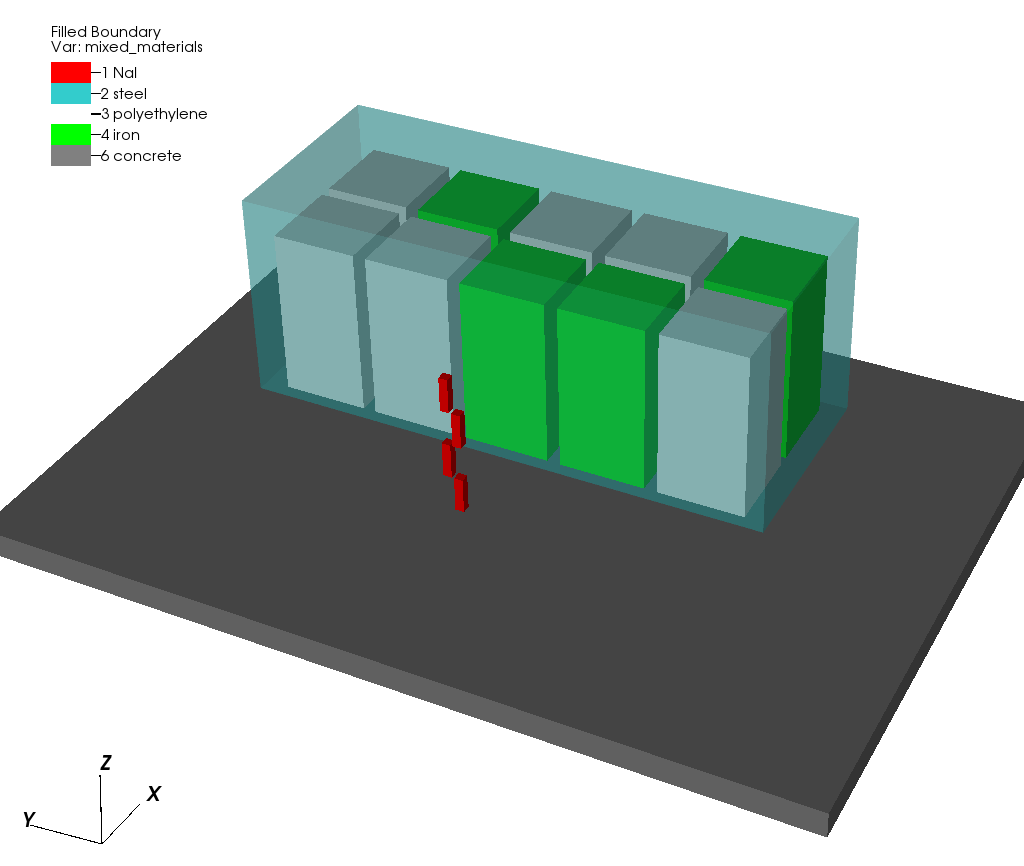
\includegraphics[width=\textwidth]{img/portal1.png}
\end{subfigure}
\begin{subfigure}{0.475\textwidth}
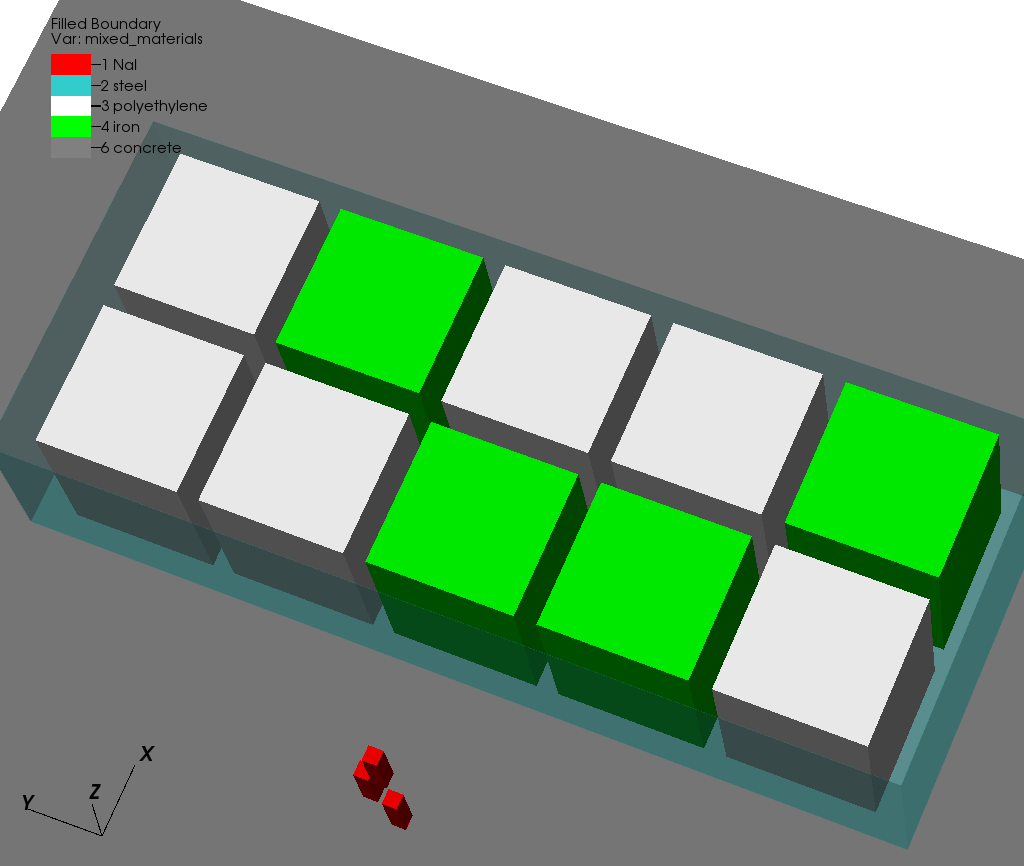
\includegraphics[width=\textwidth]{img/portal2.png}
\end{subfigure}
\caption{Top and side views of simplified portal problem \cite{advantg}.}
\label{p1}
\end{figure}

In Figure \ref{p1}, the different colors represent different materials. The NaI
detectors are red and the gray material is concrete. The two types of material
blocks are iron, shown in green, and polyethylene, shown in white. The steel
cargo container surrounds the particle source and material blocks and is a
semitransparent blue.

A non-uniform Cartesian mesh that captures all of the problem's material
boundaries was constructed for this simulation. The voxels are nominally 10 cm
thick within the cargo container. Additional mesh planes parallel to the
$x-$axis were added to the gaps between the homogenized iron and polyethylene
blocks \cite{advantg}. Vacuum boundary conditions are present at all problem
edges.

\subsection{Calculation Parameters}
\label{params}

All of the deterministic calculations used 32 processes on a 2.8GHz AMD 
Opteron\texttrademark\ 6320 Processor \cite{amd}, two for each logical CPU
unit. With this in mind, all deterministic calculations were set to use the
same Denovo computational block structure of 8 blocks in the $x-$dimension, 4
blocks in the $y-$dimension, and 1 block in the $z-$dimension;
thus the total number of computational blocks equals the number of processes.
Denovo uses the Koch-Baker-Alcouffe (KBA) parallel sweep algorithm for high
parallel efficiency in calculating transport sweeps \cite{denovo}; the
aforementioned block structure was chosen to achieve the same parallel
decomposition among all test case deterministic simulations. 

All but one of the test cases use the same coarse energy group structure
specified in the ``27n19g'' library; the groups in this library are listed in
Table A-1 of Appendix A of the ADVANTG technical report \cite{advantg}. The
exception to this is the simplified portal problem. The highest energy
emission line of Ba-133 is 383.8 keV, so weight window bounds above this
energy would not be used in the Monte Carlo simulation. Thus, the highest
energy group of the deterministic calculations was set to group number 41,
which has an upper energy of 400 keV \cite{advantg}. Because 
energy discretization is treated the same way between the traditional discrete 
ordinates formulation and the LDO equations, it was assumed that energy group 
structure would not greatly impact the comparative results.

In the deterministic calculations, forward solutions for the test cases were
generated using quadruple range (QR), Galerkin, linear-discontinuous finite 
element (LDFE), and LDO quadrature sets. All test cases were run with the same 
quadrature sets; increasing sizes of quadrature sets were used to ascertain the
angular mesh refinement necessary for a given quadrature type to converge to a 
solution. The degrees and sizes of the LDO quadrature sets used are listed in
Table \ref{ldo-n}.

\begin{table}[!htb]
\centering
\caption{Properties of LDO quadrature sets used in deterministic calculations.}
\begin{tabular}{cc}
\multicolumn{1}{l}{\textbf{Quadrature Order ($\mathbf{N}$)}} & 
\multicolumn{1}{l}{\textbf{Number of Points}} \\
\hline
3 & 16 \\
5 & 36 \\
8 & 81 \\
9 & 100 \\
11 & 144 \\
12 & 169 \\
13 & 196 \\
14 & 225 \\
\end{tabular}
\label{ldo-n}
\end{table}

QR quadrature sets were chosen to generate the reference results against which
the LDO results are compared. QR was selected because they are commonly used 
in hybrid methods for Monte Carlo variance reduction parameter generation and 
therefore provide a relevant baseline. The Exnihilo framework allows the user
to select the number of polar and azimuthal angles in each octant when using a
QR quadrature set; for these studies, the number of polar and azimuthal angles
per octant were each set to the same value, with the values ranging from one
per octant (for a total of eight angles) to nine per octant (for a total of
648 angles). 

LDFE and Galerkin quadrature sets were also chosen because of their interesting
mathematical properties. Compared to QR quadrature sets, LDFE quadrature sets
have been shown to exhibit more accurate solutions for the scalar flux in both 
simple and more complex geometry and material configurations \cite{ldfe}; they 
approximate the angular flux using direction cosines and are determined by
requiring that the integration of the related interpolation basis functions is
equal to the surface area of a unit sphere. For LDFE quadrature sets, if $N$ is
the order of the quadrature, there are $4^{(N+1)}$ angles per octant
\cite{exum}. In this work, the LDFE quadrature orders used were one (128 total
angles) and two (8192 total angles).

Galerkin quadrature sets offer several advantages relative to the standard \sn\
method for problems with highly anisotropic scattering \cite{morel}. Similar to
the LDO equations, the ``hybrid collocation-Galerkin-S$_\mathrm{N}$'' method
developed by Morel has the same algebraic structure as the traditional discrete
ordinates equations but employs a nonstandard scattering treatment. For
an \sn\ order $N$, a given Galerkin quadrature set
has a total of $N(N+2)$ angles. For reasons noted below, the Galerkin quadrature
orders used were 2 and 4; the Galerkin quadrature sets
used in this work have 8 and 24 total angles, respectively.

The step characteristics (SC) spatial discretization was used in all of the
deterministic calculations based on the recommendation listed in Section 9.1.3
of the Exnihilo user manual \cite{exum}. In the DLVN and portal monitor
scenarios, the point sources are approximated as small spherical volumetric
sources. Except for the Galerkin quadratures, all calculations used a P$_5$ scattering
expansion. At the time of this writing, Galerkin quadrature sets are
implemented in the Exnihilo framework with the restriction that the \pn\ order
be one greater than the \sn\ order. That is, for the Galerkin quadrature set of
\sn\ order 2, the corresponding \pn\ order is set equal to 3, and for the
Galerkin quadrature set of \sn\ order 4, the \pn\ order is 5.

The Monte Carlo calculations in this work were run on one Dell PowerEdge C6220
server blade node with two Intel Xeon 10-core Ivy Bridge processors (a total of
20 cores) \cite{savio}. All calculations were specified to use 21 MPI tasks; MCNP
reserves one ``master'' process for communication and transports particles with
the remaining available tasks \cite{mcnp}. So, for the purpose of parallel
efficiency, one transport process per hardware core was used here.

All of the Monte Carlo calculations were run with a fixed number of particle
histories to simulate. For the steel plate in water and simplified portal
monitor cases, all calculations used 1\E{9} particle histories in both the
CADIS and \fwc\ contexts. The DLVN experimental benchmark case was simulated
with 1\E{10} neutron histories as it was modeled after calculations in
Reference \cite{sw-dlvn}. All Monte Carlo tally results $\xbar$ are reported
with the one standard deviation confidence interval $\xbar(1\pm R)$ where the
relative error $R \equiv S_{\xbar}/\xbar$ \cite{mcnp}.

In the \fwc\ calculations for the DLVN and simplified portal monitor scenarios,
we examine Monte Carlo results corresponding to biasing parameters from a
chosen representative subset of the quadrature sets.
For these comparisons, quadrature sets of similar angular mesh
refinement were chosen such that the quadrature sets have approximately the 
same total number of angles, with the exception of the Galerkin quadrature set.
The QR quadrature set is of order 4 and has 128 angles, the LDFE set is order 1
with 128 angles, and the LDO set is of order 11 with 144 angles. 
The Galerkin quadrature set chosen as the representative example here is of
order 4 and has 24 angles. This set was chosen because its corresponding \pn\
order is 5 and so the scattering data used matches that of the other quadrature
types. 

%%---------------------------------------------------------------------------%%
\section{Results}
\label{sec:results}

For the three test case scenarios described above, we will examine the flux
tally results and Figure of Merit (FOM) values reported by MCNP. We note that
Figures of Merit are calculated as
%
\begin{equation}
\text{FOM} = \frac{1}{R^2T},
\label{eq:fom}
\end{equation}
%
where $R$ is the estimated relative error and $T$ is the computer
time taken to complete the calculation \cite{mcnp}. Flux tally and FOM values
are presented for the test case scenarios in the contexts of both the CADIS and
\fwc\ methods, with additional focus on how the results vary as a function of
angular mesh refinement used in the deterministic calculations from which Monte
Carlo variance reduction parameters were generated.

%%---------------------------------------------------------------------------%%
\subsection{Steel Plate Embedded in Water}

%%---------------------------------------------------------------------------%%
\subsubsection{CADIS}

For the CADIS calculations for the steel plate embedded in water, the adjoint
source was set to be the detector tally. Figure \ref{steel-cad-tally} shows
the MCNP-reported flux tally for the detector at the end of the steel plate
for each angular mesh refinement for each quadrature type. We note that the
Monte Carlo calculations with biasing parameters from the Galerkin quadrature set of
order 2 and the LDO quadrature set of order 5 were not able to finish in a
timely manner for the hardware configuration used in this work, so Monte Carlo
results for those two data points are not included here. The flux tally
results are plotted as a function of angular mesh refinement to demonstrate the
impact of angular mesh refinement on flux tally solution for the different
quadrature types. Figure \ref{steel-cad-tally} also includes the flux tally
value for an unbiased Monte Carlo calculation as a reference point of
comparison; it is shown as a horizontal black line with dashed lines on either
side indicating the one standard deviation confidence interval.

\begin{figure}[!hbt]
\centering
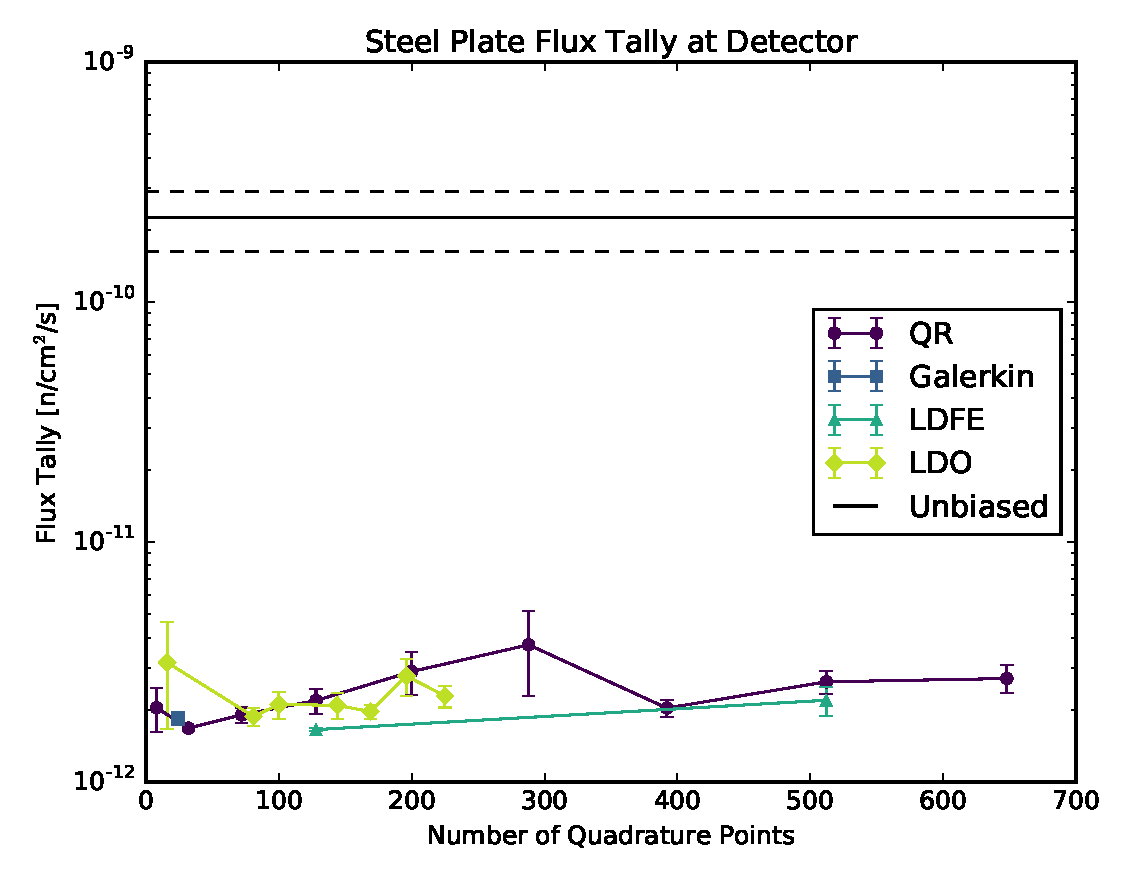
\includegraphics[max height=0.445\textheight]{img/steel-cadis-tally.eps}
\caption{MCNP-reported flux tally values at the end of the steel plate.}
\label{steel-cad-tally}
\end{figure}

All of the biased results tend towards a tally calculation on the order of
$10^{-12}$, while the unbiased tally calculation is on the order of
$10^{-10}$. This phenomenon has been previously documented
\cite{wilsonslaybaugh} and can be largely attributed to the resonances in the
iron cross section; the unresolved resonance region in the iron cross section
spans multiple energy groups, leading to inaccuracies in the discretized
multigroup cross section values used in deterministic calculations. 

While the results from this problem are incorrect, it is instructive to look
at the Figures of Merit for the various results to observe trends that could
translate to other problems where correct results are obtained. Figure 
\ref{steel-cad-fom} shows the reported FOM value for the detector tally for the
various quadrature sets and orders. We again plot the results as a function of
angular mesh refinement with a black horizontal line denoting the FOM for the
unbiased Monte Carlo calculation. The biasing parameters corresponding to the
LDFE quadrature set of order 1 result in the highest FOM value while those of
the QR set of order 1 result in the lowest FOM value. For all LDO quadrature
sets of order 8 and above, the Figures of Merit are one order of magnitude
greater than that of the unbiased calculation.

\begin{figure}[!htb]
\centering
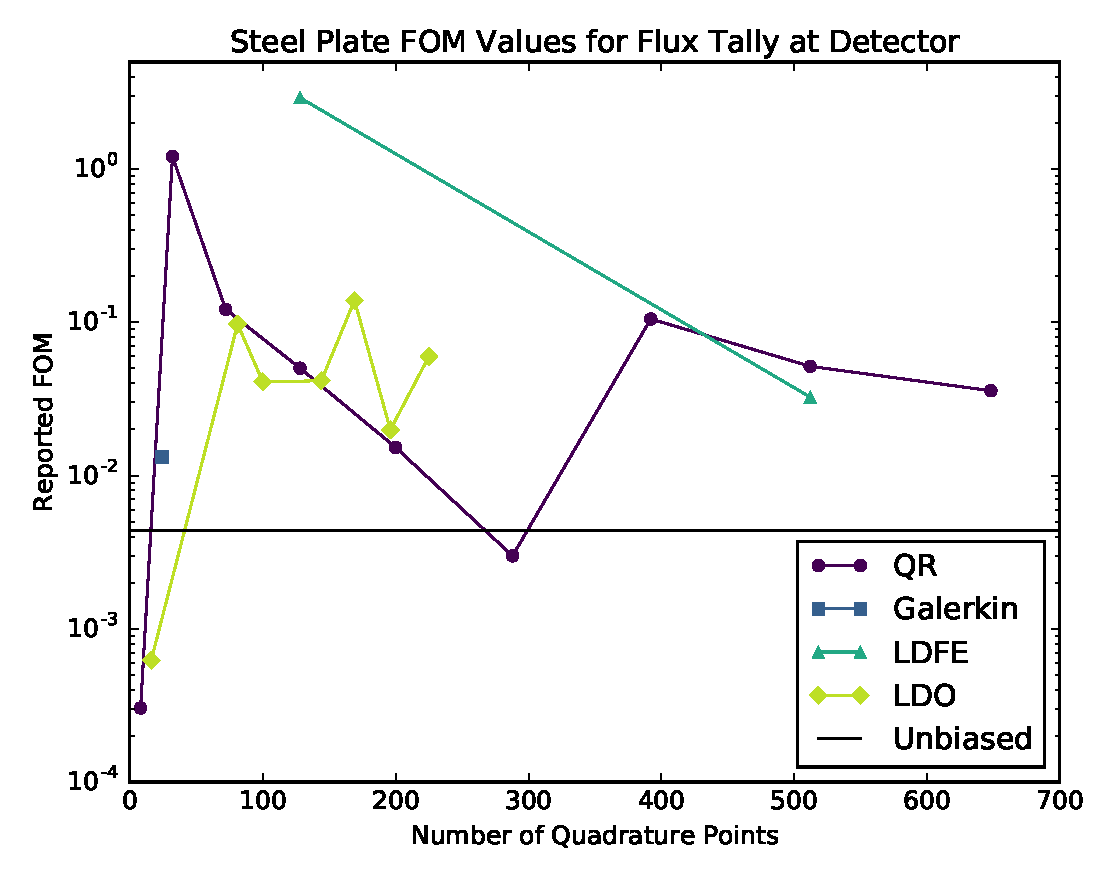
\includegraphics[max height=0.445\textheight]{img/steel-cadis-fom.eps}
\caption{FOM values for MCNP flux tally at the end of the steel plate.}
\label{steel-cad-fom}
\end{figure}

To conclude this section, we consider the overall trends in angular mesh
refinement in Figures \ref{steel-cad-tally} and \ref{steel-cad-fom}. It
appears that the angular mesh refinement does not have a large impact on the
flux tally value in this scenario, as all of the biased tally results fall
within the same order of magnitude and do not exhibit any trends as a function
of the number of discrete angles used. The Figures of Merit vary somewhat
more greatly. Specifically, the LDO biasing parameters appear to gather around
FOM values of 0.005 even as the number of discrete angles used is increased.
So, for the steel plate in water problem solved with the CADIS
method, one could use a relatively low-order (i.e., order 8) LDO quadrature
set to generate Monte Carlo biasing parameters that result in a Figure of
Merit comparable to (and better than most of, as seen here) those produced by
finer angular meshes.

\FloatBarrier
%%---------------------------------------------------------------------------%%
\subsubsection{\fwc}

For the \fwc\ calculations for the steel plate in water, the adjoint source was
set to be a mesh tally over all of the air beyond the steel plate. The
discretization for the adjoint source mesh tally is the same as that listed in 
Section \ref{sec:steel_params}\ Specifically, the adjoint source mesh is
identical to the overall problem mesh in the $x-$ and $y-$directions but starts
at $z = 130$ cm and extends to the problem boundary at $z = 140$ cm.
The Monte Carlo calculation with biasing parameters from the Galerkin quadrature set
of order 2 was not able to finish in a timely manner for the hardware
configuration used in this work, so Monte Carlo results for this data point
are not included here.

Figure \ref{steel-fwc-tally} shows the total tally summed over all air in the
problem for the biased and unbiased calculations. The biased calculations are
plotted as a function of angular mesh refinement and the unbiased calculation
value is shown as a black horizontal line. Like the CADIS method, the \fwc\
method generates biasing parameters such that the biased Monte Carlo flux
tally results all fall far below that of the unbiased calculation. Similarly,
in this case, the angular mesh refinement has little impact on the tally
result. If using an LDO quadrature set to generate biasing parameters with
the \fwc\ method in a similar scenario, a low-order LDO angular mesh could be
used to good effect.

\begin{figure}[!htb]
\centering
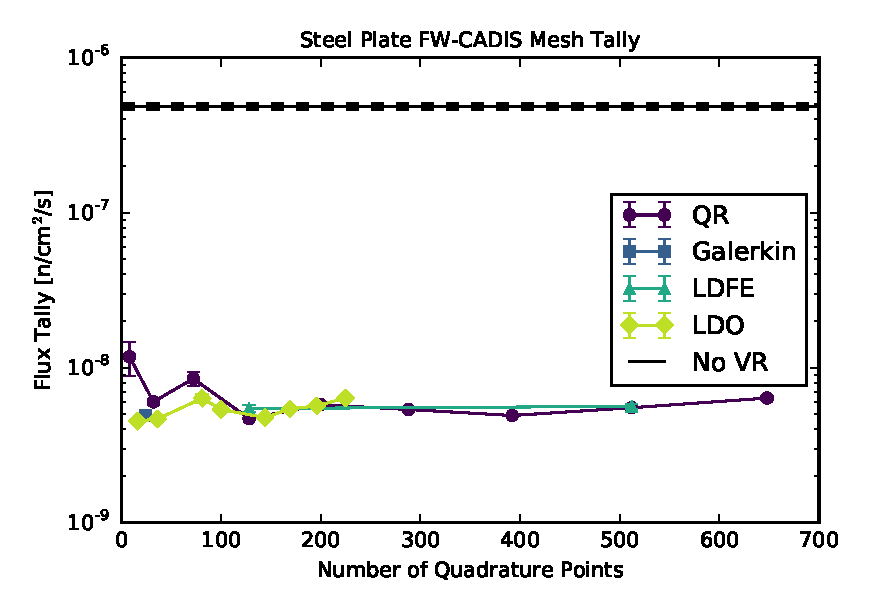
\includegraphics[max height=0.445\textheight]{img/steel-fwcadis-tally.eps}
\caption{Flux tally over the air region in the steel plate test with the \fwc\ method.}
\label{steel-fwc-tally}
\end{figure}

To analyze the performance of the representative quadrature sets' variance
reduction parameters for the steel plate in water case using the \fwc\ method,
we will look at the average FOM values over the entire adjoint source mesh
tally. The Figures of Merit were calculated by taking the average relative
error over all spatial cells in the air block mesh tally and using that mean
value in combination with the MCNP-reported computer time and Equation
\eqref{eq:fom}. Figure \ref{steel-fwc-fom} shows these average Figures of Merit
as a function of the number of angles used in generating the biasing
parameters. The average FOM for the unbiased calculation is shown as a
horizontal black line.

\begin{figure}[!htb]
\centering
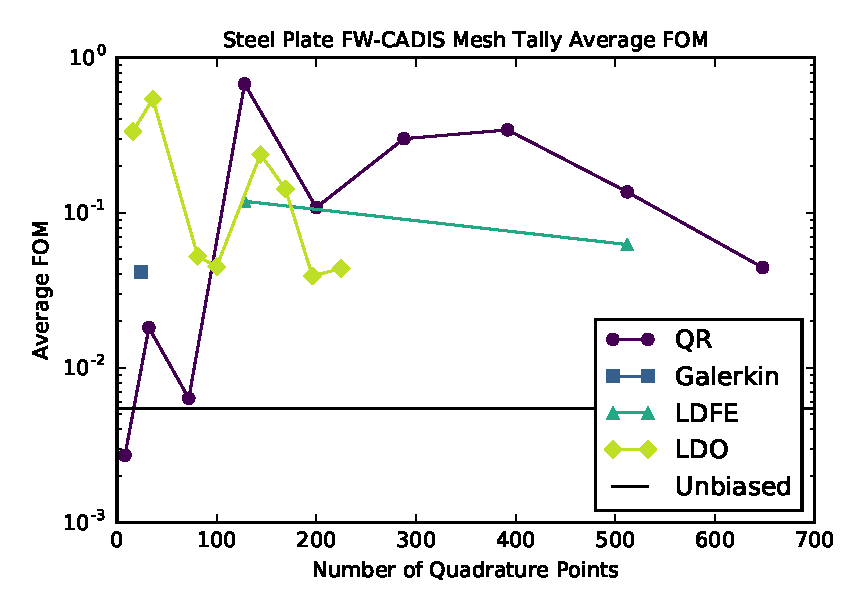
\includegraphics[max height=0.445\textheight]{img/steel-fwcadis-fom.eps}
\caption{Average FOM values for the mesh tally in the \fwc\ steel plate scenario.}
\label{steel-fwc-fom}
\end{figure}

We see a different trend here in that the highest average FOM values tend to
come from quadrature sets with mid-range angular mesh refinement; the coarsest
and finest angular meshes produce Monte Carlo biasing parameters that result
in reduced Figures of Merit. Considering Figures \ref{steel-fwc-tally} and
\ref{steel-fwc-fom}, we note that one would wish to use a lower-order (e.g.,
order 5) LDO quadrature set to generate variance reduction parameters for a
Monte Carlo mesh tally using the \fwc\ method.

\FloatBarrier
%%---------------------------------------------------------------------------%%
\subsection{Dog-Legged Void Neutron (DLVN)}

%%---------------------------------------------------------------------------%%
\subsubsection{CADIS}

To study the DLVN problem in the context of the CADIS method, the adjoint
source was set to be the tally located at detector \#14 in the original
experiment. Figure \ref{dlvn-cad-tally} shows the MCNP-reported tally for the
forward scalar flux at the location of detector \#14. Here we see that all of
the biased calculation values fall within the error of the unbiased result.
However, all of these tally calculations (biased and unbiased) do not match
the experimentally calculated flux value of 2.74\E{-7} $\pm$ 5\% n/cm$^2$/s
at detector \#14.

\begin{figure}[!htb]
\centering
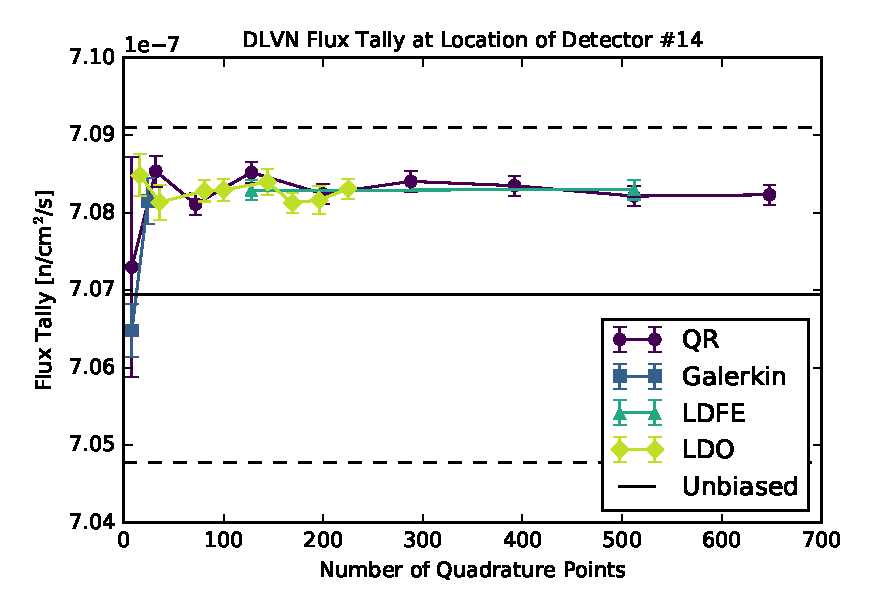
\includegraphics[max height=0.445\textheight]{img/dlvn-cadis-tally.eps}
\caption{Flux tally at detector \#14 in the DLVN problem with the CADIS method.}
\label{dlvn-cad-tally}
\end{figure}

\begin{figure}[!htb]
\centering
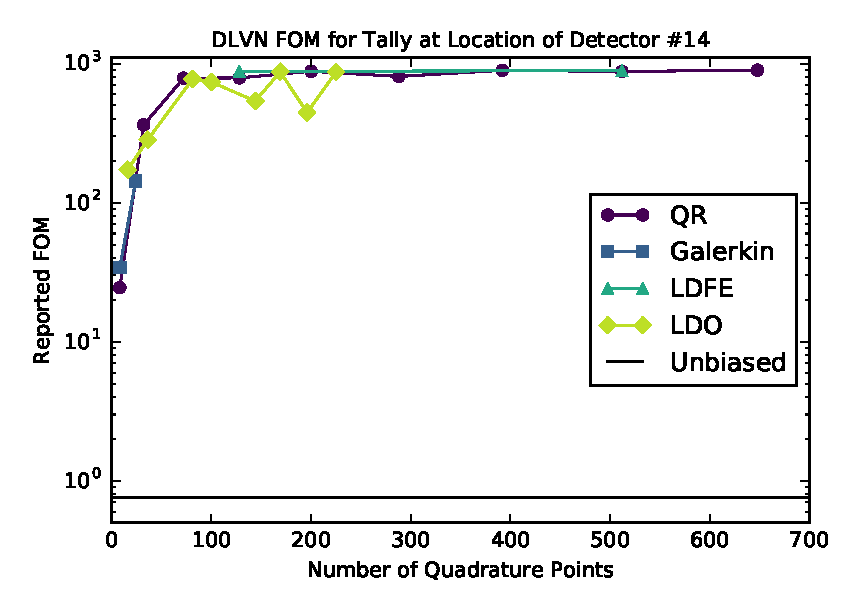
\includegraphics[max height=0.445\textheight]{img/dlvn-cadis-fom.eps}
\caption{FOM values for the DLVN problem detector \#14 tally with the CADIS 
         method.}
\label{dlvn-cad-fom}
\end{figure}

Figures \ref{dlvn-cad-tally} and \ref{dlvn-cad-fom} show similar convergence
behavior with respect to angular mesh refinement for the biased tally
calculations and Figure of Merit values. Beyond the lowest-order angular mesh
refinement for each quadrature type studied here, the tally result for this
detector location using the CADIS method is not impacted by further refining
the angular mesh. The Figures of Merit for the tally calculations reach a
similar upper bound, but this happens more slowly with respect to angular mesh
refinement for the LDO quadrature sets. Like the tally in the steel plate case
above, the LDO quadrature set of order 8 is the optimal choice with respect to
flux tally result and FOM value for detector \#14 in the DLVN experimental
benchmark problem in the CADIS context.

\FloatBarrier
%%---------------------------------------------------------------------------%%
\subsubsection{\fwc}

Considering the DLVN case with the \fwc\ method, the adjoint source was
specified to be the combination of all of the detector locations in the
problem.

Figures \ref{dlvn-fwc-5} and \ref{dlvn-fwc-9} exhibit the same lack of trend in
flux tally as a function of angular mesh refinement. That is, in general, for
detector locations \#5 and \#9, using more discrete angles in the \fwc\
deterministic calculations does not greatly impact the flux tally result from
MCNP. Figures \ref{dlvn-fwc-13} and \ref{dlvn-fwc-14} show similar behavior
with the exception of the most coarse angular meshes. For these detector
locations, any angular mesh refinement other than the coarsest angular mesh
will produce a consistent forward scalar flux tally result. Figures
\ref{dlvn-fwc-11} and \ref{dlvn-fwc-12} show slightly more variation in flux
tally result with angular mesh refinement. These two detector locations'
tallies have also higher statistical error relative to those at the other
detector locations. Overall, though, the flux tallies at detectors \#11 and
\#12 are not heavily impacted by the refinement of the angular mesh used in
generating the Monte Carlo biasing parameters, but a mid-range number of
quadrature points should be used to avoid the large statistical errors seen at
the extreme ends of the angular mesh refinement spectrum.

Like their corresponding flux tally graphs, Figures \ref{dlvn-fwc-5},
\ref{dlvn-fwc-9}, and \ref{dlvn-fwc-13} show almost no variation in FOM with
angular mesh refinement for the tallies at detector locations \#5, \#9, and
\#13. This is to be expected, considering the uniform statistical error and
stable flux tally results at these locations. Figure \ref{dlvn-fwc-11} shows
variation in FOM with angular mesh refinement that is more varied, which
corresponds to the larger statistical uncertainties in the flux tally values
for detector \#11. Figure \ref{dlvn-fwc-12} shows little variation in FOM with
angular mesh refinement with the exception of the finest QR set. Lastly,
\ref{dlvn-fwc-14} shows an upper FOM limit of approximately 200 across all
quadrature types, with the Figure of Merit largely consistent across
quadrature types with the exception of QR angular meshes.

In Table \ref{dlvn-fwc-det} we compare the Monte Carlo forward flux tally
results for the representative quadrature sets listed in Section \ref{params}\
Results from the unbiased Monte Carlo calculation are also included for
comparison. All Monte Carlo flux tally values are reported with an uncertainty
of one standard deviation. For all detector locations, the Monte Carlo flux
tallies do not match the experimentally measured flux values for any of the
representative quadrature sets or the unbiased calculation, so we only compare
the Monte Carlo calculations in this table. We do note that the Monte Carlo
calculations overestimate the flux tally at all detector locations with the
exception of detector \#13. The flux tallies at detectors 5, 9, 13, and 14 all
match within statistical uncertainty for all of the Monte Carlo calculations.
At detector \#11, the biased Monte Carlo calculations match within standard
error, but the calculations using the QR and LDO biasing parameter fall outside
of the error bounds of the unbiased calculation. Somewhat similarly, at
detector \#14, all of the biased calculations match one another within
statistical uncertainty, but they are all outside of the error bounds of the
unbiased flux tally calculation.

\begin{table}[!htb]
\centering
\scriptsize
\caption{DLVN benchmark flux tallies [n/cm$^2$/s] calculated with \fwc.}
\label{dlvn-fwc-det}
\begin{tabular}{l|ccccc}
         & \textbf{QR} & \textbf{Galerkin} & \textbf{LDFE} 
         & \textbf{LDO} & \textbf{Unbiased}  \\ \hline
 Det. \#5 & \mr{1.3341 $\pm$ 0.0003} & \mr{1.3344 $\pm$ 0.0003} & \mr{1.3347 $\pm$ 0.0004} &
            \mr{1.3344 $\pm$ 0.0003} & \mr{1.3315 $\pm$ 0.0092} \rule{0pt}{2.6ex} \\
    (\E{-7})      &    &   &  &   &    \\
 Det. \#9 & \mr{2.5225 $\pm$ 0.0005} & \mr{2.5224 $\pm$ 0.0005} & \mr{2.5229 $\pm$ 0.0004} &
            \mr{2.2555 $\pm$ 0.0004} & \mr{2.5104 $\pm$ 0.0127} \rule{0pt}{2.6ex}  \\
   (\E{-7}) &   &  &  &  &   \\
 Det. \#11 & \mr{1.4420 $\pm$ 0.0005} & \mr{1.4451 $\pm$ 0.0027} & \mr{1.4446 $\pm$ 0.0026} &
            \mr{1.4463 $\pm$ 0.0015} & \mr{1.4463 $\pm$ 0.0010} \rule{0pt}{2.6ex} \\
   (\E{-5}) &   &  &  &  &   \\
 Det. \#12 & \mr{2.4749 $\pm$ 0.0004} & \mr{2.4743 $\pm$ 0.0004} & \mr{2.4751 $\pm$ 0.0004} &
            \mr{2.4744 $\pm$ 0.0004} & \mr{2.4684 $\pm$ 0.0042}  \rule{0pt}{2.6ex} \\
    (\E{-6}) &   &  &  &  &   \\
 Det. \#13 & \mr{4.3984 $\pm$ 0.0011} & \mr{4.3997 $\pm$ 0.0011} & \mr{4.3994 $\pm$ 0.0011} &
            \mr{4.3983 $\pm$ 0.0011} & \mr{4.4170 $\pm$ 0.0175}  \rule{0pt}{2.6ex} \\
    (\E{-7}) &   &  &  &  &   \\
 Det. \#14 & \mr{7.0070 $\pm$ 0.0025} & \mr{7.0829 $\pm$ 0.0045} & \mr{7.0813 $\pm$ 0.0026} &
            \mr{7.0834 $\pm$ 0.0032} & \mr{7.0694 $\pm$ 0.0216}  \rule{0pt}{2.6ex} \\
    (\E{-7}) &   &  &  &  &   \\ \hline
\end{tabular}
\end{table}

To examine the FOM values in a more quantifiable way, Table 
\ref{dlvn-fwc-fom-table} lists the FOM values for all detector locations for
each of the representative quadrature sets as well as the unbiased calculation.
The maximum FOM value in each detector location column is emphasized. Of the
six detector locations, the representative LDO quadrature set achieves the
highest FOM for two of the locations. The representative QR quadrature set is
the only other type to also deliver the highest Figure of Merit for two out of
six detectors; the Galerkin and LDFE quadrature set biasing parameters each
only achieve the highest FOM for one detector location. So, the representative
LDO quadrature set's biasing parameters perform comparably to those from the
representative QR quadrature set with respect to obtaining high FOM values for
multiple detector locations using the \fwc\ method for the DLVN problem.

\begin{table}[!hbt]
\centering
\caption{\fwc\ FOM values for representative quadratures for the DLVN problem.}
\label{dlvn-fwc-fom-table}
\begin{tabular}{l|cccccc}
\multicolumn{1}{l|}{Quad. Type}
& \multicolumn{1}{l}{Det. \#5}
& \multicolumn{1}{l}{Det. \#9}
& \multicolumn{1}{l}{Det. \#11}
& \multicolumn{1}{l}{Det. \#12}
& \multicolumn{1}{l}{Det. \#13}
& \multicolumn{1}{l}{Det. \#14}
\\ \hline
\begin{tabular}[c]{@{}l@{}}   QR \end{tabular} 
& \begin{tabular}[c]{@{}c@{}} 483.012 \end{tabular} % fom for #5
& \begin{tabular}[c]{@{}c@{}} 709.51 \end{tabular} % fom for #9
& \begin{tabular}[c]{@{}c@{}} \textbf{202.66} \end{tabular} % fom for #11
& \begin{tabular}[c]{@{}c@{}} 747.914 \end{tabular} % fom for #12
& \begin{tabular}[c]{@{}c@{}} 380.843 \end{tabular} % fom for #13
& \begin{tabular}[c]{@{}c@{}} \textbf{185.40} \end{tabular} % fom for #14
\\
\begin{tabular}[c]{@{}l@{}}   Galerkin \end{tabular} 
& \begin{tabular}[c]{@{}c@{}} \textbf{527.794} \end{tabular} % fom for #5
& \begin{tabular}[c]{@{}c@{}} 649.88 \end{tabular} % fom for #9
& \begin{tabular}[c]{@{}c@{}} 5.9934 \end{tabular} % fom for #11
& \begin{tabular}[c]{@{}c@{}} 798.878 \end{tabular} % fom for #12
& \begin{tabular}[c]{@{}c@{}} 326.107 \end{tabular} % fom for #13
& \begin{tabular}[c]{@{}c@{}} 52.098 \end{tabular} % fom for #14
\\
\begin{tabular}[c]{@{}l@{}}   LDFE \end{tabular} 
& \begin{tabular}[c]{@{}c@{}} 310.276 \end{tabular} % fom for #5
& \begin{tabular}[c]{@{}c@{}} 710.43 \end{tabular} % fom for #9
& \begin{tabular}[c]{@{}c@{}} 6.6749 \end{tabular} % fom for #11
& \begin{tabular}[c]{@{}c@{}} 926.278 \end{tabular} % fom for #12
& \begin{tabular}[c]{@{}c@{}} \textbf{391.624} \end{tabular} % fom for #13
& \begin{tabular}[c]{@{}c@{}} 166.51 \end{tabular} % fom for #14
\\
\begin{tabular}[c]{@{}l@{}}   LDO \end{tabular}
& \begin{tabular}[c]{@{}c@{}} 478.242 \end{tabular} % fom for #5
& \begin{tabular}[c]{@{}c@{}} \textbf{721.22} \end{tabular} % fom for #9
& \begin{tabular}[c]{@{}c@{}} 19.959 \end{tabular} % fom for #11
& \begin{tabular}[c]{@{}c@{}} \textbf{943.959} \end{tabular} % fom for #12
& \begin{tabular}[c]{@{}c@{}} 369.423 \end{tabular} % fom for #13
& \begin{tabular}[c]{@{}c@{}} 110.40 \end{tabular} % fom for #14
\\
Unbiased  & 0.149122 & 0.27845 & 14.555 & 2.52563 & 0.453763 & 0.76362
\end{tabular}
\end{table}

In summary, for test case scenarios such as the DLVN problem in which the
\fwc\ method is used to generate Monte Carlo variance reduction parameters to
optimize the response at multiple flux tally detector locations, a relatively
coarse quadrature set of any of the types studied here can be used to
sufficient effect. However, the coarsest available quadrature sets should be
avoided; flux tally results and Figures of Merit for the various detector
locations tend to level out as a function of angular mesh refinement beyond
the quadrature sets with the fewest number of angles. In particular, if using
an LDO quadrature set in another similar scenario, we would suggest using a
point set of order 5 or 8.

\begin{figure}[!htb]
\begin{subfigure}{\linewidth}
\centering
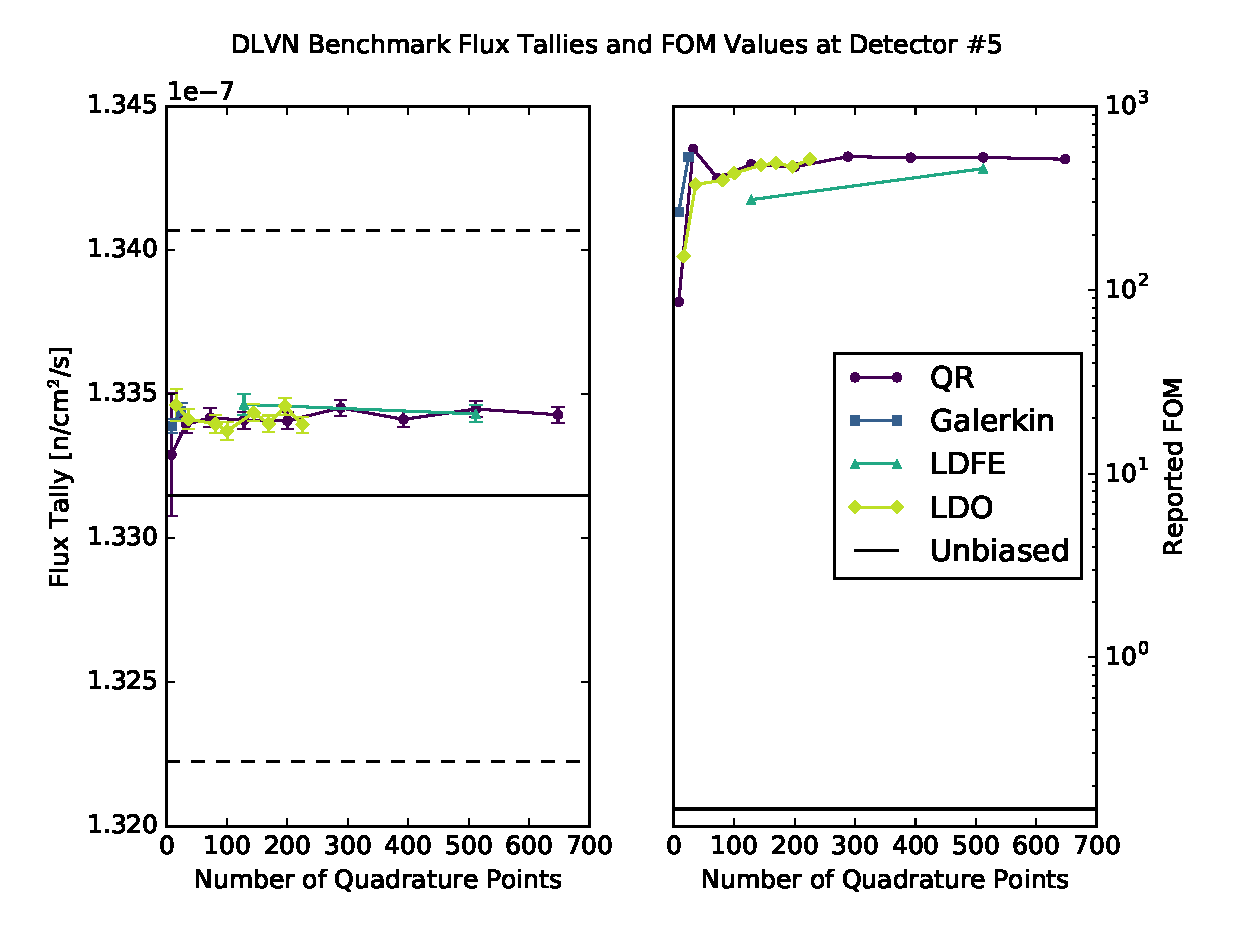
\includegraphics[max height=0.445\textheight]
{img/dlvn-fwcadis-5.eps}
\subcaption{MCNP-reported forward flux tally and FOM values at detector \#5.}
\label{dlvn-fwc-5}
\end{subfigure} 
\\
\begin{subfigure}{\linewidth}
\centering
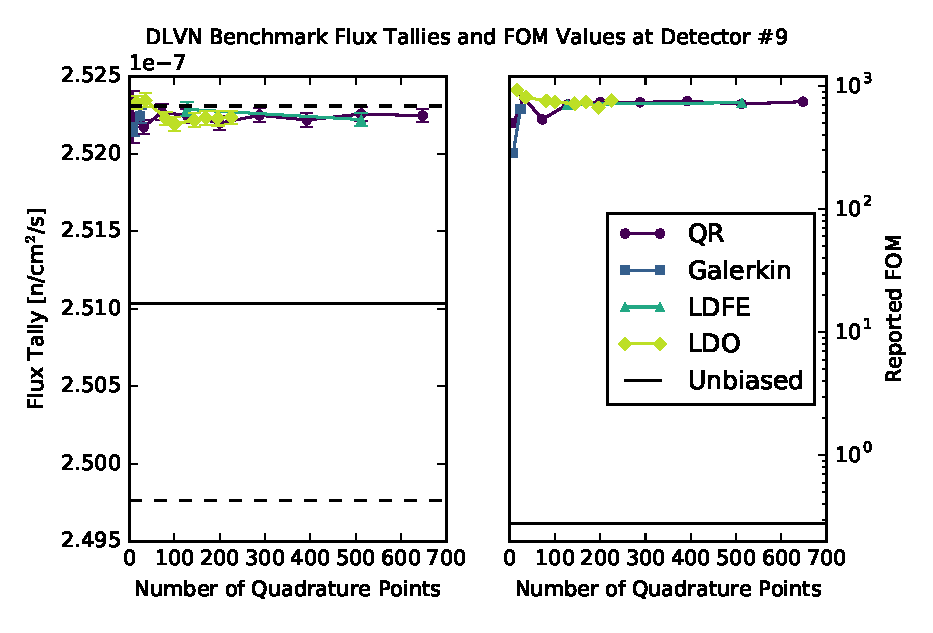
\includegraphics[max height=0.445\textheight]
{img/dlvn-fwcadis-9.eps}
\subcaption{MCNP-reported forward flux tally and FOM values at detector \#9.}
\label{dlvn-fwc-9}
\end{subfigure}
\end{figure}
\clearpage
\begin{figure}[!htb]
\ContinuedFloat
\begin{subfigure}{\linewidth}
\centering
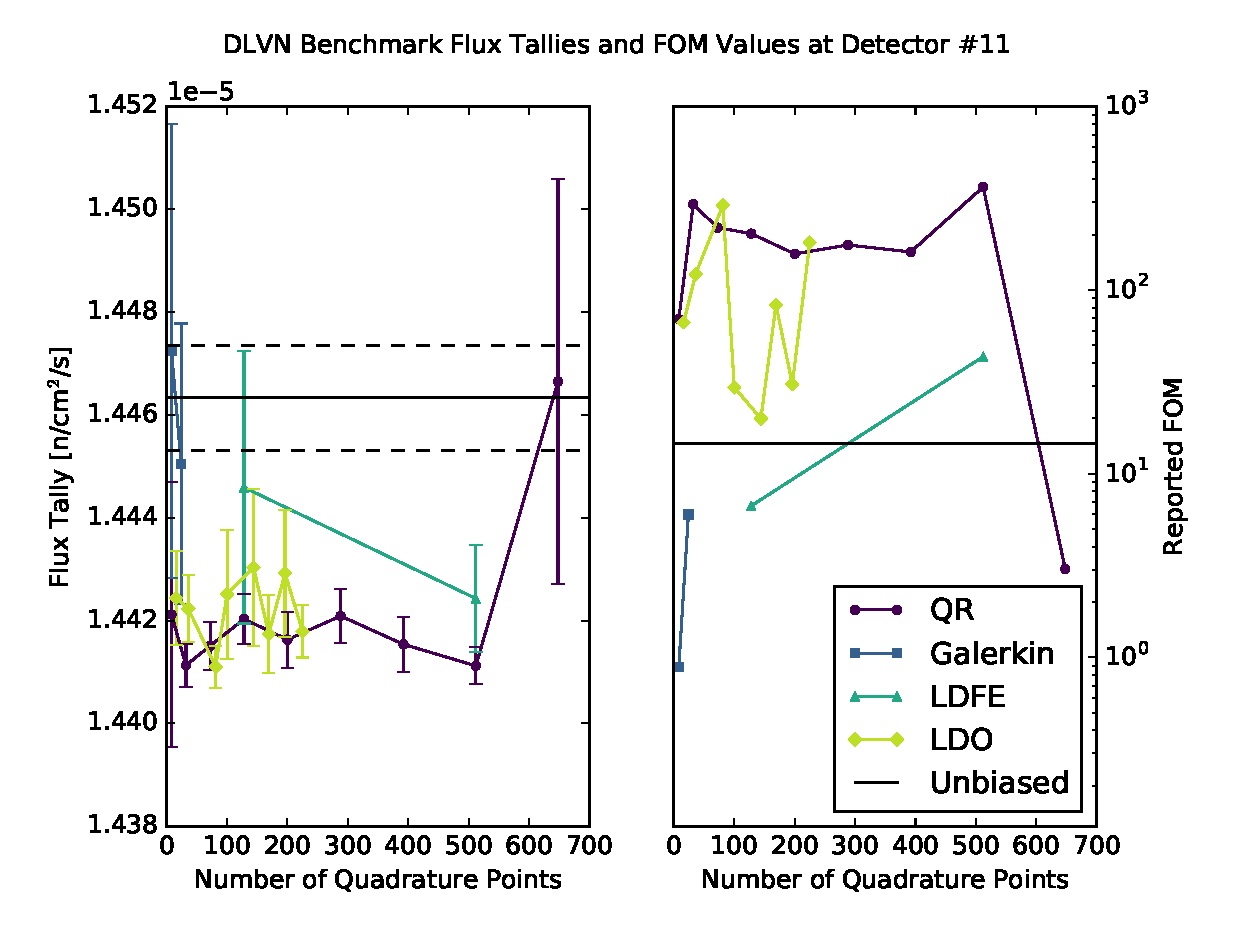
\includegraphics[max height=0.445\textheight]
{img/dlvn-fwcadis-11.eps}
\subcaption{MCNP-reported forward flux tally and FOM values at detector \#11.}
\label{dlvn-fwc-11}
\end{subfigure}
\\
\begin{subfigure}{\linewidth}
\centering
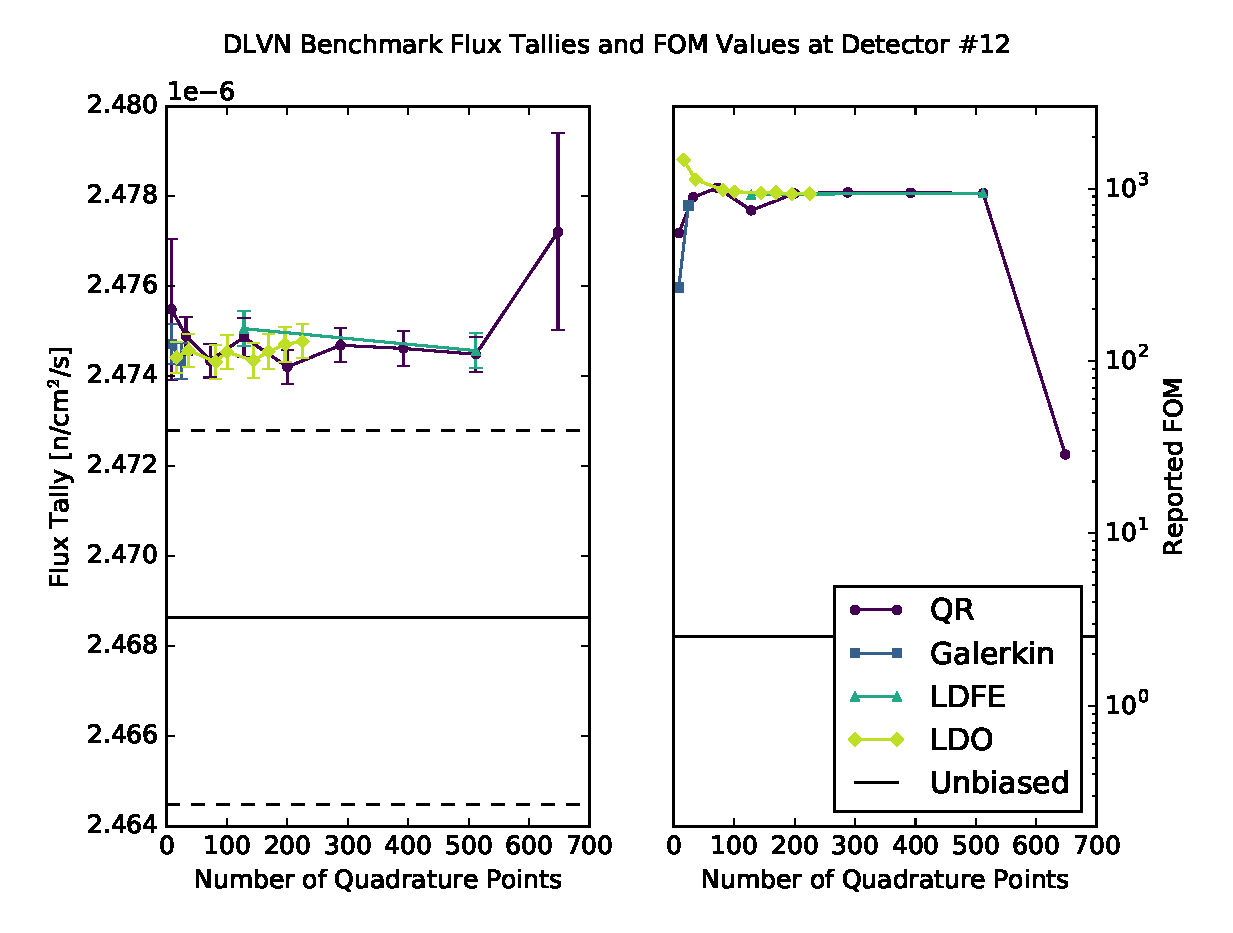
\includegraphics[max height=0.445\textheight]
{img/dlvn-fwcadis-12.eps}
\subcaption{MCNP-reported forward flux tally and FOM values at detector \#12.}
\label{dlvn-fwc-12}
\end{subfigure}
\end{figure}
\clearpage
\begin{figure}[!htb]
\ContinuedFloat
\begin{subfigure}{\linewidth}
\centering
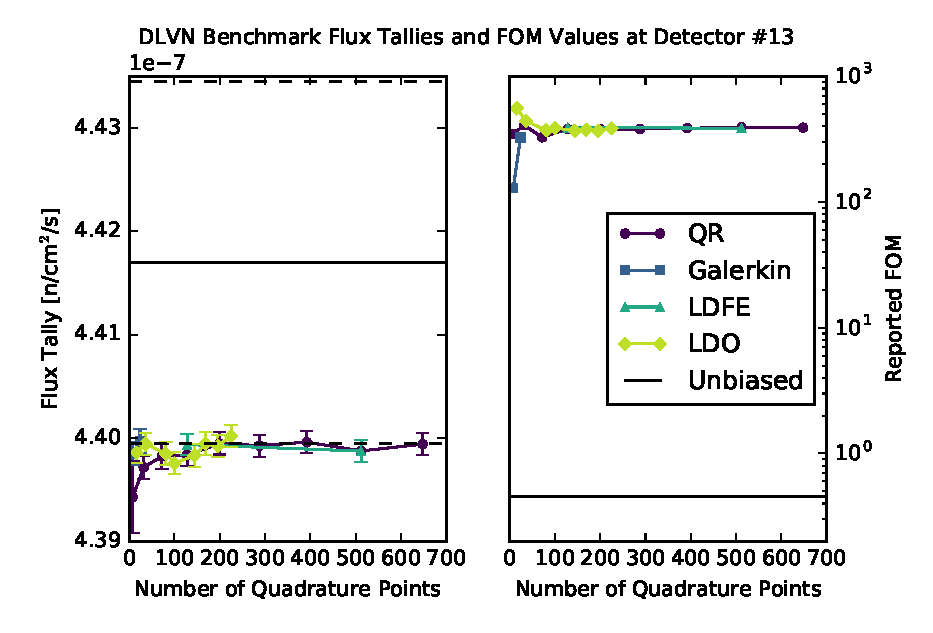
\includegraphics[max height=0.445\textheight]
{img/dlvn-fwcadis-13.eps}
\subcaption{MCNP-reported forward flux tally and FOM values at detector \#13.}
\label{dlvn-fwc-13}
\end{subfigure} 
\\
\begin{subfigure}{\linewidth}
\centering
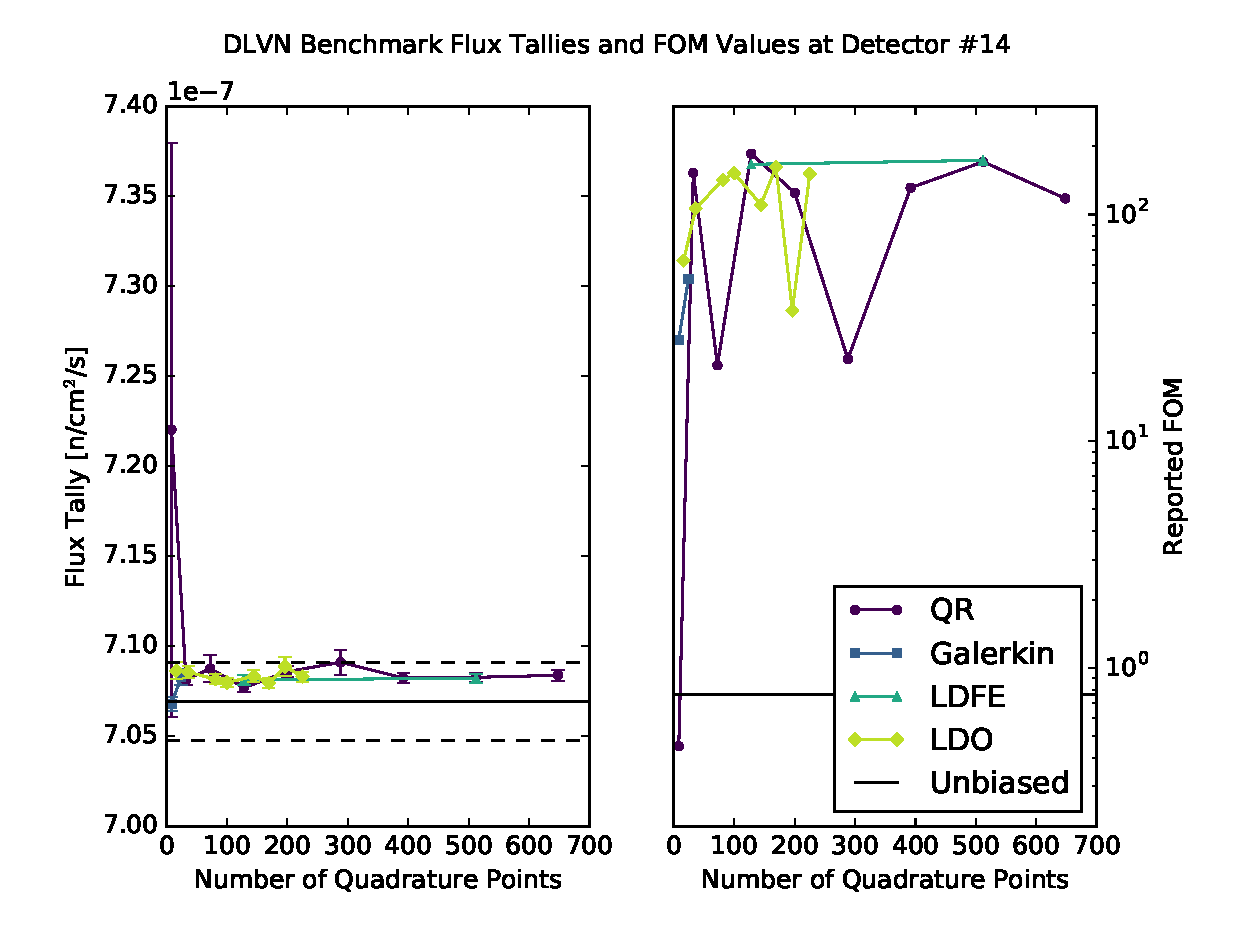
\includegraphics[max height=0.445\textheight]
{img/dlvn-fwcadis-14.eps}
\subcaption{MCNP-reported forward flux tally and FOM values at detector \#14.}
\label{dlvn-fwc-14}
\end{subfigure}
\caption{\fwc\ flux tallies and FOM values for the DLVN problem.}
\label{dlvn-fwc-tally}
\end{figure}

\FloatBarrier
%%---------------------------------------------------------------------------%%
\subsection{Simplified Portal Monitor}

%%---------------------------------------------------------------------------%%
\subsubsection{CADIS}

To study calculations for the simplified portal monitor scenario in the context
of the CADIS method, the adjoint source was set to be the top detector in the
small array.

Figures \ref{cargo-cad-tally} and \ref{cargo-cad-fom} show the MCNP-reported
forward scalar flux tally values and Figures of Merit, respectively. As with
the other test cases, the values are plotted as a function of the number of
quadrature points used to generate the biasing parameters in order to explore
the impact of angular mesh refinement on flux tally and FOM.

\begin{figure}[!htb]
\centering
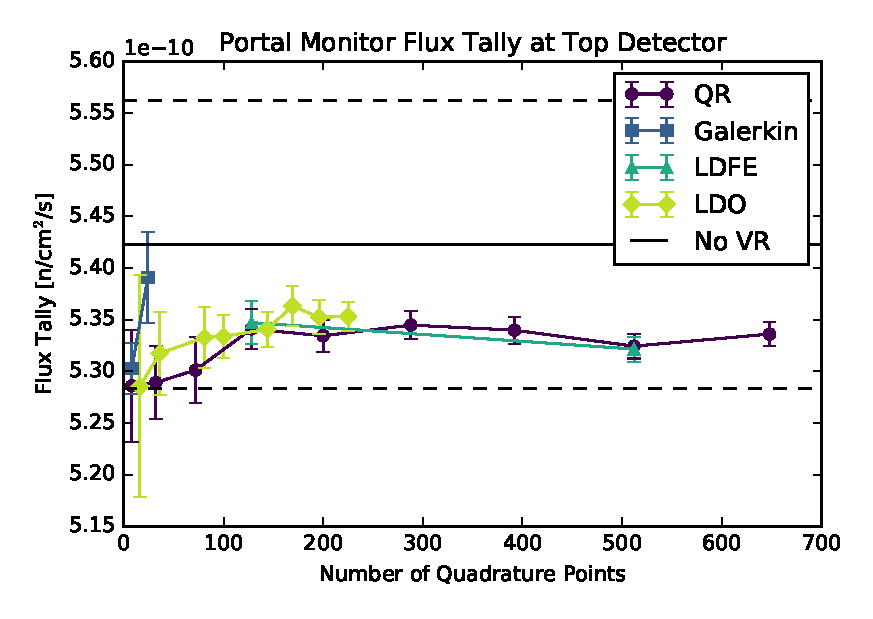
\includegraphics[max height=0.445\textheight]{img/portal-cadis-tally.eps}
\caption{Flux tally in the portal monitor top detector using the CADIS method.}
\label{cargo-cad-tally}
\end{figure}

\begin{figure}[!htb]
\centering
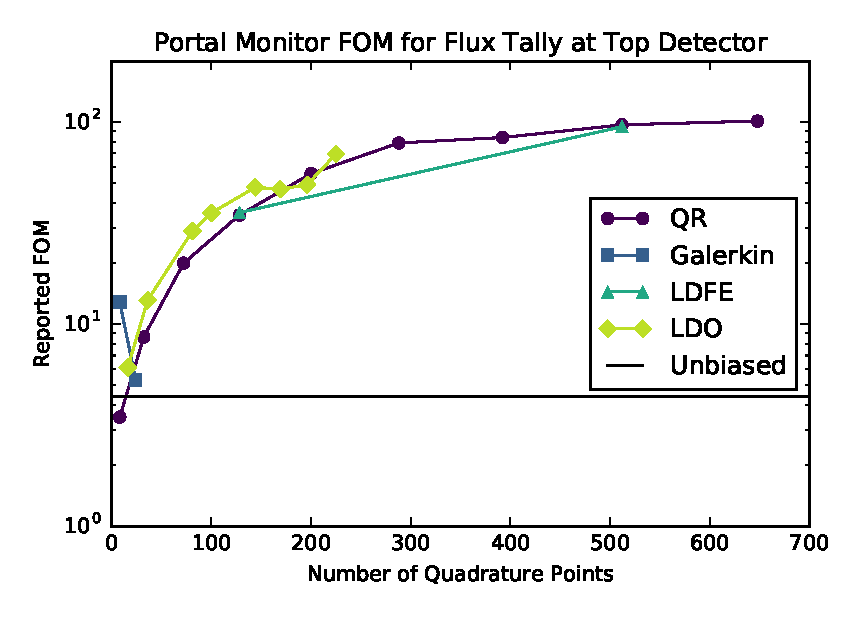
\includegraphics[max height=0.445\textheight]{img/portal-cadis-fom.eps}
\caption{CADIS method FOM values for the portal monitor top detector flux tally.}
\label{cargo-cad-fom}
\end{figure}

Similar to other test cases, the flux tally values reported in Figure 
\ref{cargo-cad-tally} show a trend of converging to a stable value after the
first few coarsest angular meshes. The flux tally values from the biased
calculations all fall within the statistical error of that of the unbiased
calculation but appear to require a minimum value of approximately 100
discrete angular values in order to stabilize. Figure \ref{cargo-cad-fom}
shows a strong correlation between the number of quadrature points and the
flux tally FOM, eventually approaching an upper limit around 100. The LDO
Figures of Merit increase most rapidly with the number of quadrature points
used, so one would want to use a higher-order LDO quadrature set to generate
Monte Carlo biasing parameters.

\FloatBarrier
%%---------------------------------------------------------------------------%%
\subsubsection{\fwc}

To generate Monte Carlo variance reduction parameters for the simplified portal
monitor using the \fwc\ method, the adjoint source was set to be all four
detector locations in the problem's detector array.

Figure \ref{cargo-fwc} shows MCNP-reported forward scalar flux tallies and
Figures of Merit for all four detectors in the array. The flux tallies and FOM
values are each plotted as a function of the number of discrete angles used in
the quadrature sets that were used to generate biasing parameters. In all
plots, the unbiased calculation result is shown as a horizontal black line. At
all detector locations, the forward flux tallies and FOM values show the same
trend of leveling off to a stable value once the angular mesh used for the
\fwc\ biasing parameters has been refined past the few coarsest numbers of
discrete angles. At all detector locations except for the \nth{2} in the array,
the unbiased calculation and the calculations with biasing parameters resultant
from the representative quadrature sets all match within statistical
uncertainty. The \nth{2} detector sees all representative biased flux tallies
matching one another but outside the error bounds of the unbiased flux tally
calculation.

Table \ref{cargo-fwc-fom-table} lists the Figures of Merit for the various
detector locations for the representative quadrature sets. The unbiased
calculation FOM values are also tabulated for reference. We see that the
biasing parameters from the representative LDO quadrature set produce the
highest Figures of Merit for three out of four detector locations, with the
representative QR quadrature set's biasing parameters achieving the highest FOM
for the bottom detector in the array.

\begin{table}[!hbt]
\centering
\small
\caption{\fwc\ FOM values for representative quadratures for the portal monitor.}
\label{cargo-fwc-fom-table}
\begin{tabular}{l|cccc}
\multicolumn{1}{l|}{Quad. Type}
& \multicolumn{1}{l}{Top Detector}
& \multicolumn{1}{l}{\nth{2} Detector}
& \multicolumn{1}{l}{\nth{3} Detector}
& \multicolumn{1}{l}{Bottom Detector}
\\ \hline
\begin{tabular}[c]{@{}l@{}}   QR \end{tabular} 
& \begin{tabular}[c]{@{}c@{}} 76.1145 \end{tabular} % fom for #14
& \begin{tabular}[c]{@{}c@{}} 121.241 \end{tabular} % fom for #24
& \begin{tabular}[c]{@{}c@{}} 128.9 \end{tabular} % fom for #34
& \begin{tabular}[c]{@{}c@{}} \textbf{81.125} \end{tabular} % fom for #44
\\
\begin{tabular}[c]{@{}l@{}}   Galerkin \end{tabular} 
& \begin{tabular}[c]{@{}c@{}} 30.2458 \end{tabular} % fom for #14
& \begin{tabular}[c]{@{}c@{}} 38.1391 \end{tabular} % fom for #24
& \begin{tabular}[c]{@{}c@{}} 34.01 \end{tabular} % fom for #34
& \begin{tabular}[c]{@{}c@{}} 29.016 \end{tabular} % fom for #44
\\
\begin{tabular}[c]{@{}l@{}}   LDFE \end{tabular} 
& \begin{tabular}[c]{@{}c@{}} 65.6132 \end{tabular} % fom for #14
& \begin{tabular}[c]{@{}c@{}} 96.1557 \end{tabular} % fom for #24
& \begin{tabular}[c]{@{}c@{}} 115.5 \end{tabular} % fom for #34
& \begin{tabular}[c]{@{}c@{}} 61.655 \end{tabular} % fom for #44
\\
\begin{tabular}[c]{@{}l@{}}   LDO \end{tabular} 
& \begin{tabular}[c]{@{}c@{}} \textbf{85.7067} \end{tabular} % fom for #14
& \begin{tabular}[c]{@{}c@{}} \textbf{132.962} \end{tabular} % fom for #24
& \begin{tabular}[c]{@{}c@{}} \textbf{140.3} \end{tabular} % fom for #34
& \begin{tabular}[c]{@{}c@{}} 75.135 \end{tabular} % fom for #44
\\
Unbiased & 4.40963 & 3.15204 & 2.096 & 2.8313
\end{tabular}
\end{table}

To conclude, using LDO quadrature sets to generate Monte Carlo biasing
parameters in the \fwc\ method is particularly promising for cases such as the
simplified portal monitor scenario. When selecting an LDO quadrature set to
generate variance reduction parameters for similar photon transport problems,
a relatively coarse angular mesh of order 5 or 8 may be used to good effect.

\begin{figure}[!htb]
\begin{subfigure}{\textwidth}
\centering
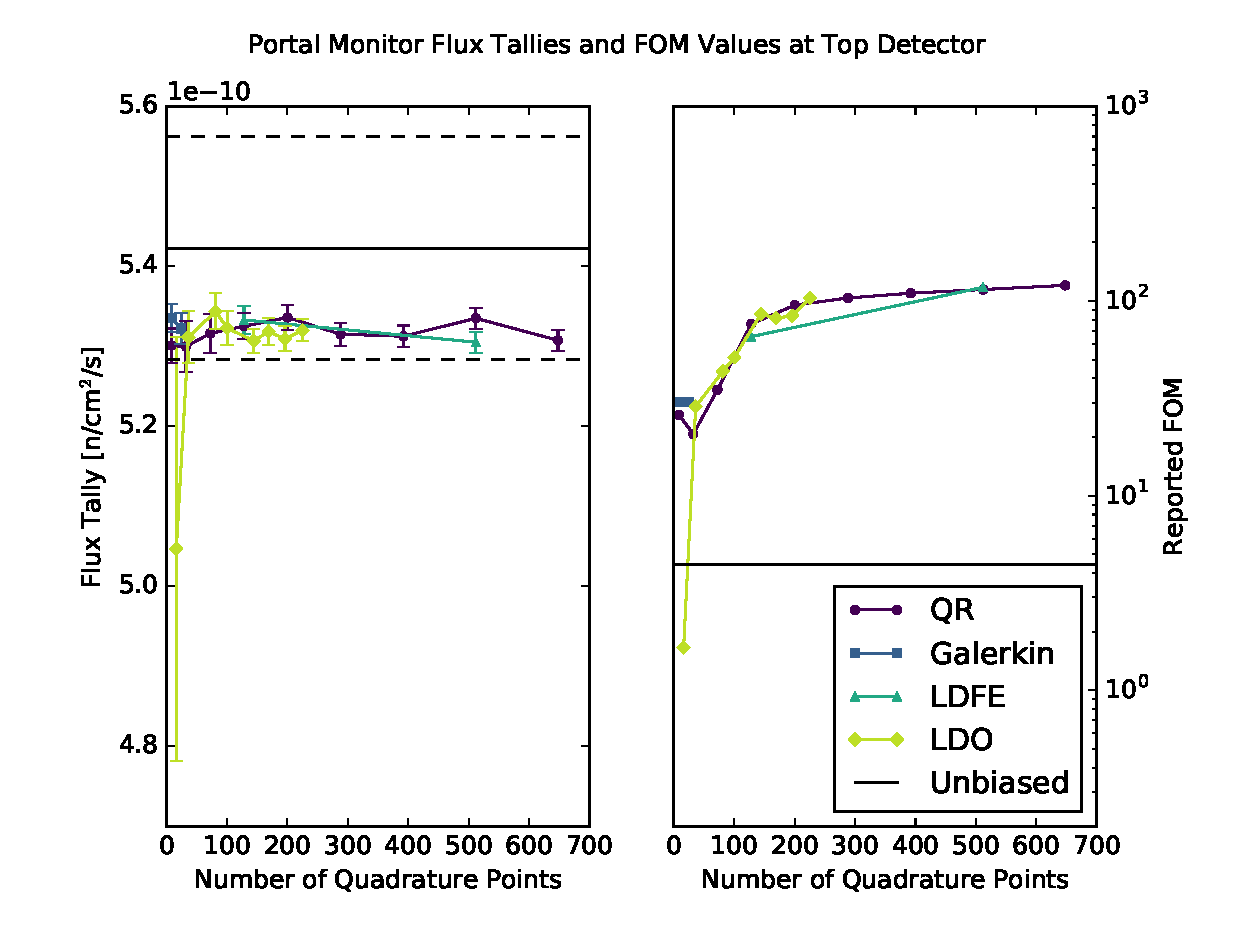
\includegraphics[max height=0.445\textheight]
{img/portal-fwcadis-1.eps}
\subcaption{MCNP-reported forward flux tally and FOM values at the top detector.}
\end{subfigure}
\\
\begin{subfigure}{\textwidth}
\centering
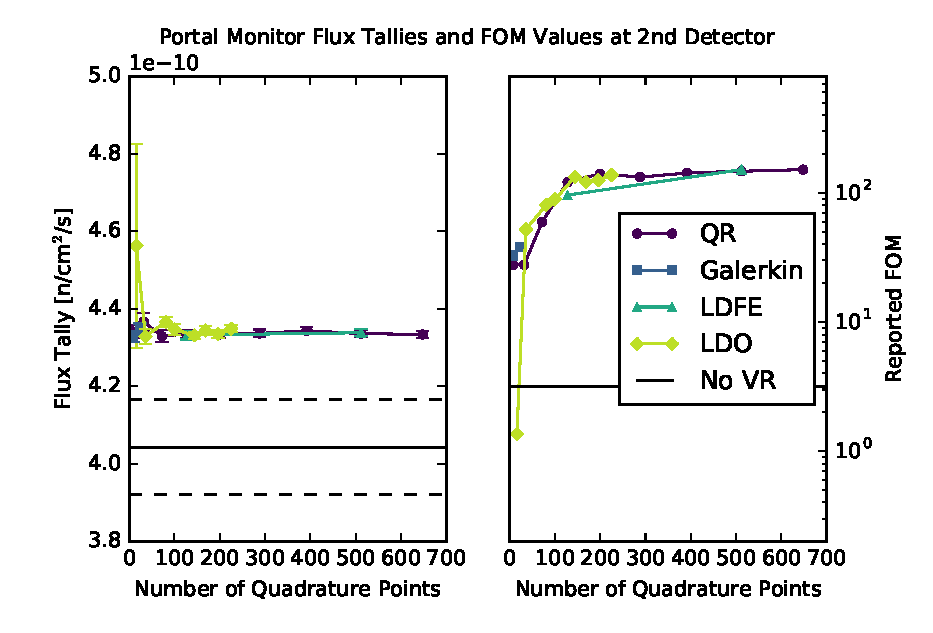
\includegraphics[max height=0.445\textheight]
{img/portal-fwcadis-2.eps}
\subcaption{MCNP-reported forward flux tally and FOM values at the second detector.}
\end{subfigure}
\end{figure}
\clearpage
\begin{figure}[!htb]
\ContinuedFloat
\begin{subfigure}{\textwidth}
\centering
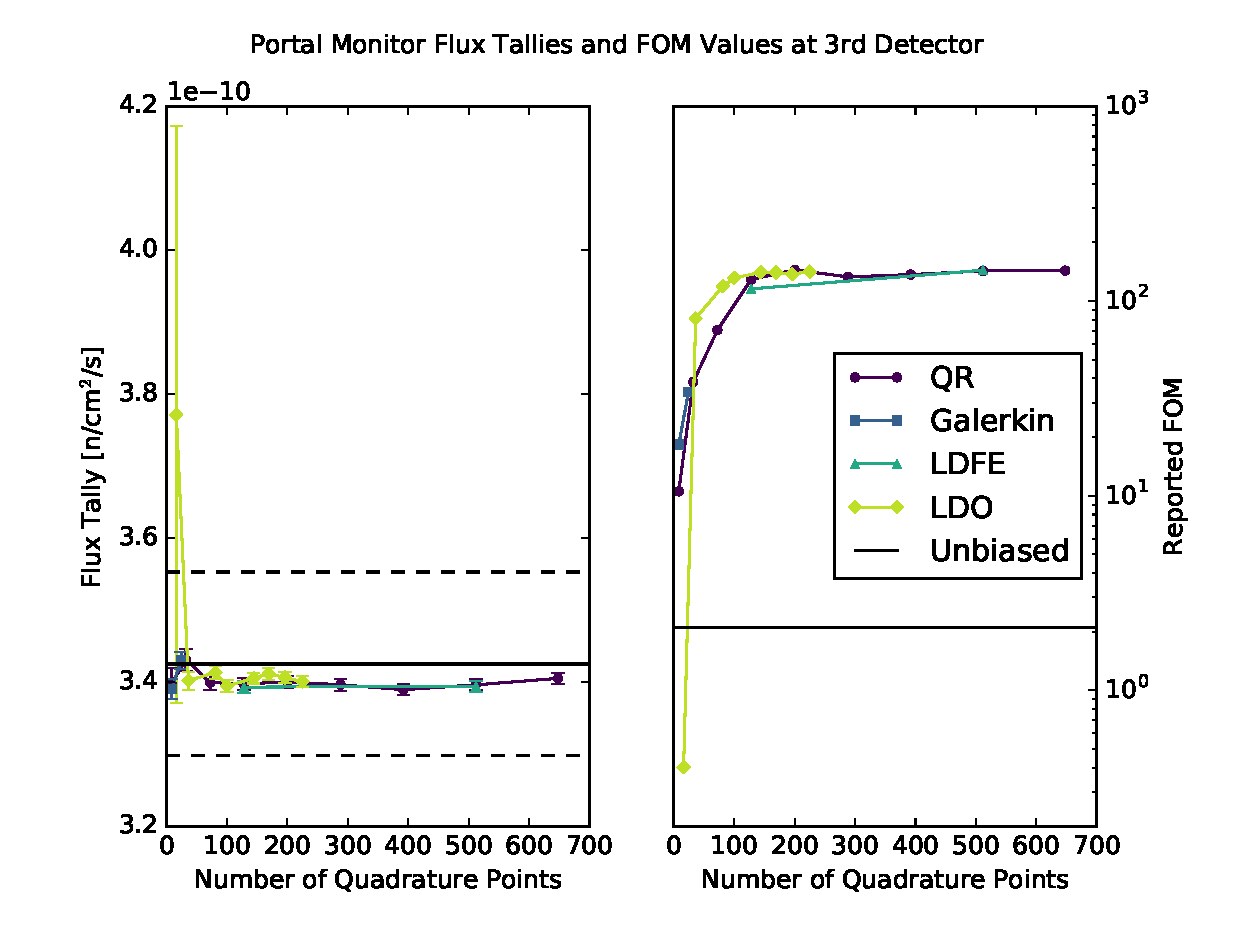
\includegraphics[max height=0.445\textheight]
{img/portal-fwcadis-3.eps}
\subcaption{MCNP-reported forward flux tally and FOM values at the third detector.}
\end{subfigure}
\\
\begin{subfigure}{\textwidth}
\centering
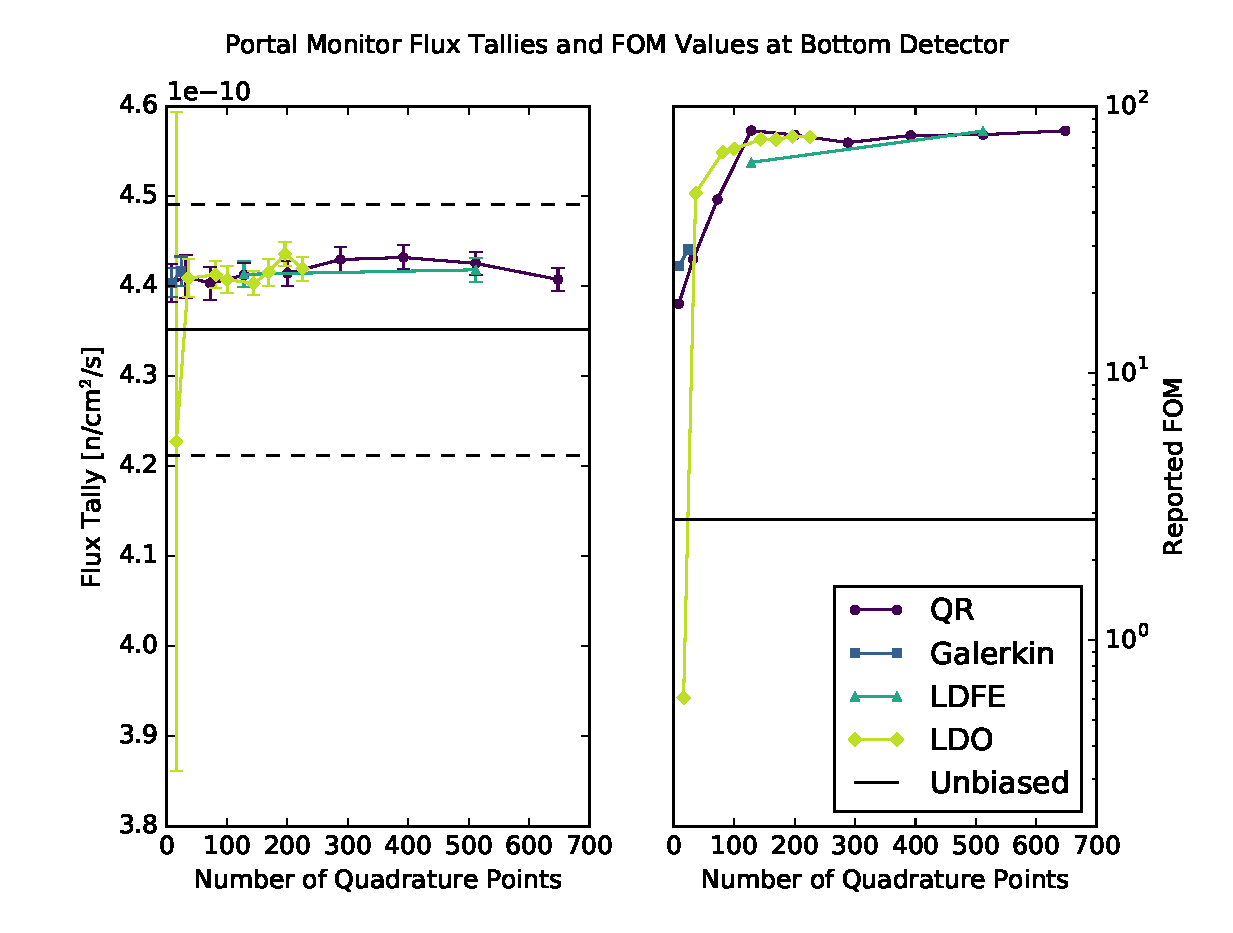
\includegraphics[max height=0.445\textheight]
{img/portal-fwcadis-4.eps}
\subcaption{MCNP-reported forward flux tally and FOM values at the bottom detector.}
\end{subfigure}
\caption{\fwc\ flux tallies and FOM values for the portal monitor scenario.}
\label{cargo-fwc}
\end{figure}

\FloatBarrier
%%---------------------------------------------------------------------------%%
\subsection{Summary}

On the whole, little correlation was seen between angular mesh refinement and
the MCNP-reported forward flux tally values in the CADIS context. If using an
LDO quadrature set to generate biasing parameters in this context for any of
the neutron transport scenarios, a low-order (3 - 8) quadrature set may be used
to sufficient effect for flux tally value and FOM achievement. For generating
biasing parameters in the CADIS context for a photon problem with an LDO
quadrature set, the finest available angular mesh should be used. This is
consistent with what is expected based on the difference between neutron and
photon scattering in the materials in these test case scenarios.

In the context of the \fwc\ method, we found that low-order (5 or 8) angular
meshes are sufficient to produce forward flux tally and Figure of Merit values
comparable to those of more refined angular meshes when using LDO quadrature
sets. The superior FOM values resultant from the representative LDO quadrature
set for three of four detectors in the simplified portal monitor scenario
begets interest in further exploration of LDO equations' solutions as input for
Monte Carlo biasing parameters for photon transport in the \fwc\ context.

%---------------------------------------------------------------------------%%
\section{Conclusions and Future Work}
\label{sec:conclusions}

The LDO equations saw their best-performing Monte Carlo biasing parameters in
the \fwc\ context. For the DLVN experimental benchmark, LDO variance reduction
parameters generated the highest Figures of Merit for two of the six detector
locations in the assembly. Of those studied here, the only other quadrature
type to achieve this was the QR quadrature set. In the case of the simplified
portal monitor scenario studied in the \fwc\ context, the LDO biasing
parameters attained the highest FOM values for three out of four detector
locations. Considering results from the test case scenarios in which neutrons
were transported using the CADIS and \fwc\ methods, we suggest a coarse
angular mesh for Monte Carlo variance reduction parameter generation based on
flux solutions resultant from solving the LDO equations. For photon transport
problems, a more refined LDO angular mesh is recommended for generating Monte
Carlo biasing parameters and achieving detector responses with high Figures of
Merit.

In general, the LDO formulation is most useful in the specific context of
Monte Carlo variance parameter generation using the \fwc\ method for photon
transport problems. It is also effective in the \fwc\ method for neutron
transport problems, though somewhat less so. However, the LDO representation
is currently limited in applicability by its current implementation in the
Exnihilo framework and the ADVANTG software. The problem space available to
explore is limited to those with vacuum boundary conditions and isotropic
fixed particle sources with non-zero volume. Adopting the LDO formulation in
another radiation transport and Monte Carlo variance reduction parameter
generation framework would be of interest if the framework is flexible in
allowing for asymmetric quadrature sets to be used and if the framework allows
for relative ease in implementing the unique features of the LDO
representation such as interpolation in angle.

\pagebreak
\section*{Acknowledgments}

This material is based upon work supported under an Integrated
University Program Graduate Fellowship as well as supported by the Department 
of Energy under Award Number(s) DE-NE0008661. This report was prepared as an
account of work sponsored by an agency of the United States Government.
Neither the United States Government nor any agency thereof, nor any of their
employees, makes any warranty, express or limited, or assumes any legal
liability or responsibility for the accuracy, completeness, or usefulness of
any information, apparatus, product, or process disclosed, or represents that
its use would not infringe privately owned rights. Reference herein to any 
specific commercial product, process, or service by trade name, trademark, 
manufacturer, or otherwise does not necessarily constitute or imply its 
endorsement, recommendation, or favoring by the United States Government or
any agency thereof. The views and opinions of authors expressed herein do not 
necessarily state or reflect those of the United States Government or any 
agency thereof. This research used the Savio computational cluster resource 
provided by the Berkeley Research Computing program at the University of 
California, Berkeley (supported by the UC Berkeley Chancellor, Vice Chancellor
for Research, and Chief Information Officer).

\pagebreak

\bibliographystyle{nse}
\bibliography{ldo-mc-vr}

\end{document}

